\documentclass[12pt]{report}

\usepackage[a4paper,
			inner = 35mm,
			outer = 25mm,
			top = 25mm,
			bottom = 25mm]{geometry}
\usepackage{lmodern}
\usepackage[magyar]{babel}
\usepackage[utf8]{inputenc}
\usepackage[T1]{fontenc}
\usepackage[hidelinks]{hyperref}
\usepackage{graphicx}
\usepackage{amssymb}
\usepackage{setspace}
\usepackage[nottoc,numbib]{tocbibind}
\usepackage{amsthm}
\usepackage{minted}
\usepackage{mdframed}
\usepackage{etoolbox}
\usepackage{xcolor}



% \setcounter{secnumdepth}{3}
\onehalfspacing

\newtheorem{mydef}{Definició}
\newtheorem{mytetel}{Tétel}
\newtheorem{mylemma}{Lemma}

\BeforeBeginEnvironment{minted}{\begin{mdframed}[backgroundcolor=bg, hidealllines=true]}
\AfterEndEnvironment{minted}{\end{mdframed}}

\newcommand{\cmd}[1]{\colorbox{gray!10}{\strut #1}}

\definecolor{bg}{rgb}{0.95,0.95,0.95}
\newminted[mintedJson]{js}{breaklines, breaksymbolleft=\quad}
\newminted[mintedBash]{bash}{breaklines, breaksymbolleft=\quad}



\begin{document}

\begin{titlepage}
	\begin{center}
		\vspace*{1cm}
		
		\textbf{\LARGE 
			Forgalom igény tudatos hálózat tervezés minimális torlódással és úthosszal
		}
	
	
		\vspace{0.5cm}
	
		\textbf{\normalsize Tudáskezelő rendszerek IV. labor összefoglaló}
		
		\vfill
		
		\Large Szecsődi Imre
		
		\vspace{2.8cm}
		
		\the\year
		
	\end{center}
\end{titlepage}

\tableofcontents
	
\chapter{Bevezetés}


\section{Labor célja}

A labor célja a korábban már bemutatott cikkben\cite{avin_demand-aware_nodate} szereplő hálózat megépítése.
Az elkészült keresztrendszert kiegészíteni még egy fa építési stratégiával, ami a Véletlenszerűen felépített fa (Random fa).
Továbbá még különböző metrikák bevezetése, ami segítségével pontosabb képet kapunk arról, hogy különböző helyzetekben milyen eredményeket eredményeznek az algoritmusok.
Egy fontos megközelítésbeli változás is alkalmazva volt az algoritmus első lépésére, mennyi fát építünk és az milyen kihatással van az eredményre.

\section{Laborban megvalósított munka}

A labor ideje alatt a már elkészült keretrendszer segítségével tesztek voltak futtatva, és azok adati kiértékelve.
A keretrendszer Python \cite{noauthor_python_nodate} nyelven íródott.
A véletlen gráfok generálására a NetworkX külső csomag volt használva\cite{noauthor_networkx_nodate}.
Az adatok elemzése Python segítségével történt.

\chapter{Modell}

\section{Random fa}

Az eddigi fa építési stratégiák mindegyike valamilyen szempontból próbált egy jobb útválasztási sémát létrehozni.
A Random fa olyan megközelítést használ, hogy szimulálja azt ha valaki véletlenszerűen kötögetné össze a csomópontokat.
Az így létrehozott fák semmit nem használ olyan információt ami hatékonyabb eredményhez vezetne.
Az algoritmus a már korábban használt Sorfolytonos fára épít, azaz a csomópontokat sorfolytonosan helyezzük el.
Egyetlen változás az algoritmusban, a fához tartozó vektor ami tartalmazza a kommunikációs valószínűségeket nincs sorba rendezve, hanem ötször meg vannak benne keverve az elemek. 
Ezzel szimulálva azt, ha valaki véletlenszerűen kötögetne össze csomópontokat.


\section{Módosított fa építés}


Az cikkben szereplő cl-DAN algoritmus első lépése a csomópontok besorolása magas és alacsony halmazokba a fokszámuk alapján. 
A szerzők itt fele-fele arányban osztják el a pontokat és egy hozzáadott feltételként megnézik, hogy az alacsony fokszámúak között szerepel-e olyan csomópont, aminek a fokszáma meghaladja \(2\rho\)-t, azaz a kétszeres átlag fokszámot.

A általam módosított cl-DAN algoritmus ezt a kiegészítő szabályt veszi alapul.
Mi lenne ha, nem szabályosan fele-fele arányba lenne elosztva, hanem magán a \(2\rho\) feltételen?

Nézzünk egy példát, ahol ez jelentőséggel bír.
Tegyük fel, hogy van egy 25 csúcsú csillag gráfunk két csillaggal.
A csillag gráfban a csillag közepére kapcsolódik rá az összes másik csomópont, így van kettő 24 fokú csomópontunk, és huszonhárom darab 2 fokú csomópont. 
Az átlag fokszám így \(\rho=23\cdot2+2\cdot23=3.68\), ennek a kétszerese \(2\rho=7.36\).

Az eredeti esetben a nagy fokú csomópontokhoz a csillagok közepei fog tartozni és további tizenegy darab 2 fokú csomópont. 
Így legalább $\lceil\frac{n}{2}\rceil$ fát fogunk építeni, ahol a pontok nagy része olyan kapcsolatban van, hogy két 2 fokszámú között egy segítő csúcs van, ami hasonló hozzájuk és eredetileg 2 fokszámú volt. 
Ezzel a módszerrel jelentősen növeltük meg a torlódást a gráfban.

A módosított algoritmus az eredetivel ellenben a magas halmazban csak két darab csúcsot tartalmaz, a középpontokat.
Ezen esetben ténylegesen magas csomópontok közé helyezünk egy kisegítőt, ami bármelyik lehet a maradék 2 fokszámú csúcsok közül, ezzel redukáltuk is az épített fák számát.
%A torlódásra tekintette, meg azt tapasztalhatjuk, hogy kevesebb lesz, mintha az eredeti módszer segítségével csináltuk volna. 

A módosított algoritmus nem lesz rosszabb mint az eredeti algoritmus, mivel ott mit kiegészítő feltétel szerepel a fokszám ellenőrzés, még itt az alapot adja, így legrosszabb esetben is visszatérünk az eredetihez. 

\chapter{Tesztelés}


\section{Tesztelés menete}

A megfelelő teszt mennyiség eléréséhez véletlen szerű gráfok lettek generálva. 
Mind a három gráf típus lett tesztelésre használva, ezek paramétere pedig változott egy és tíz között.

A különböző kapacitás szimulálására a maximum fokszám meg lett határozva, hogy a 
következő halmaz elemit veheti fel $\Delta\in(10, 16, 24, 48)$.
A tesztkörnyezet támogat az átlag fokszám függvényében megadott $\Delta$ értéket. 
A tesztek segítségével ki lett mutatva, hogy egy ponton túl, már annyira nagy lesz ez az érték, hogy minden csúcs a gyökérre kapcsolódik.
Ezzel teljesen értelmét vesztve, hogy milyen fa építési stratégia volt használva, mivel a fa nem éri azt az elemszámot, hogy legyen nem direkt csatlakozó csomópont a gyökérhez. 
A \ref{delta} ábrán látható ez:  

\begin{figure}[H]
	\begin{center}
		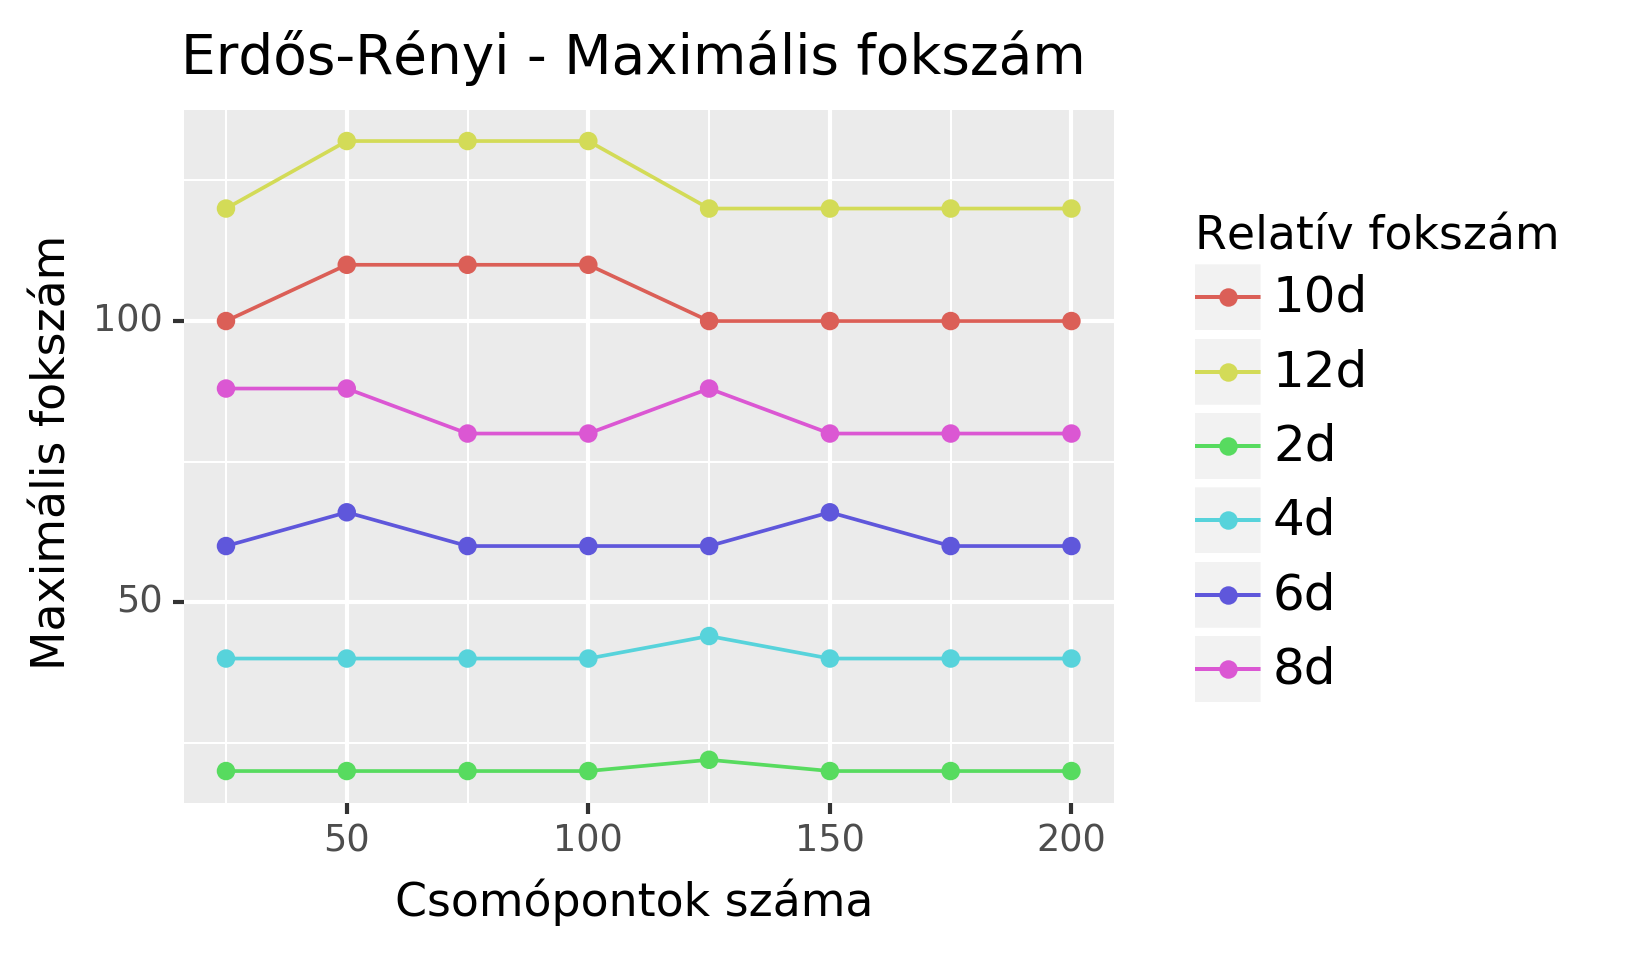
\includegraphics[width=0.49\linewidth]{pictures/delta_max.png}
		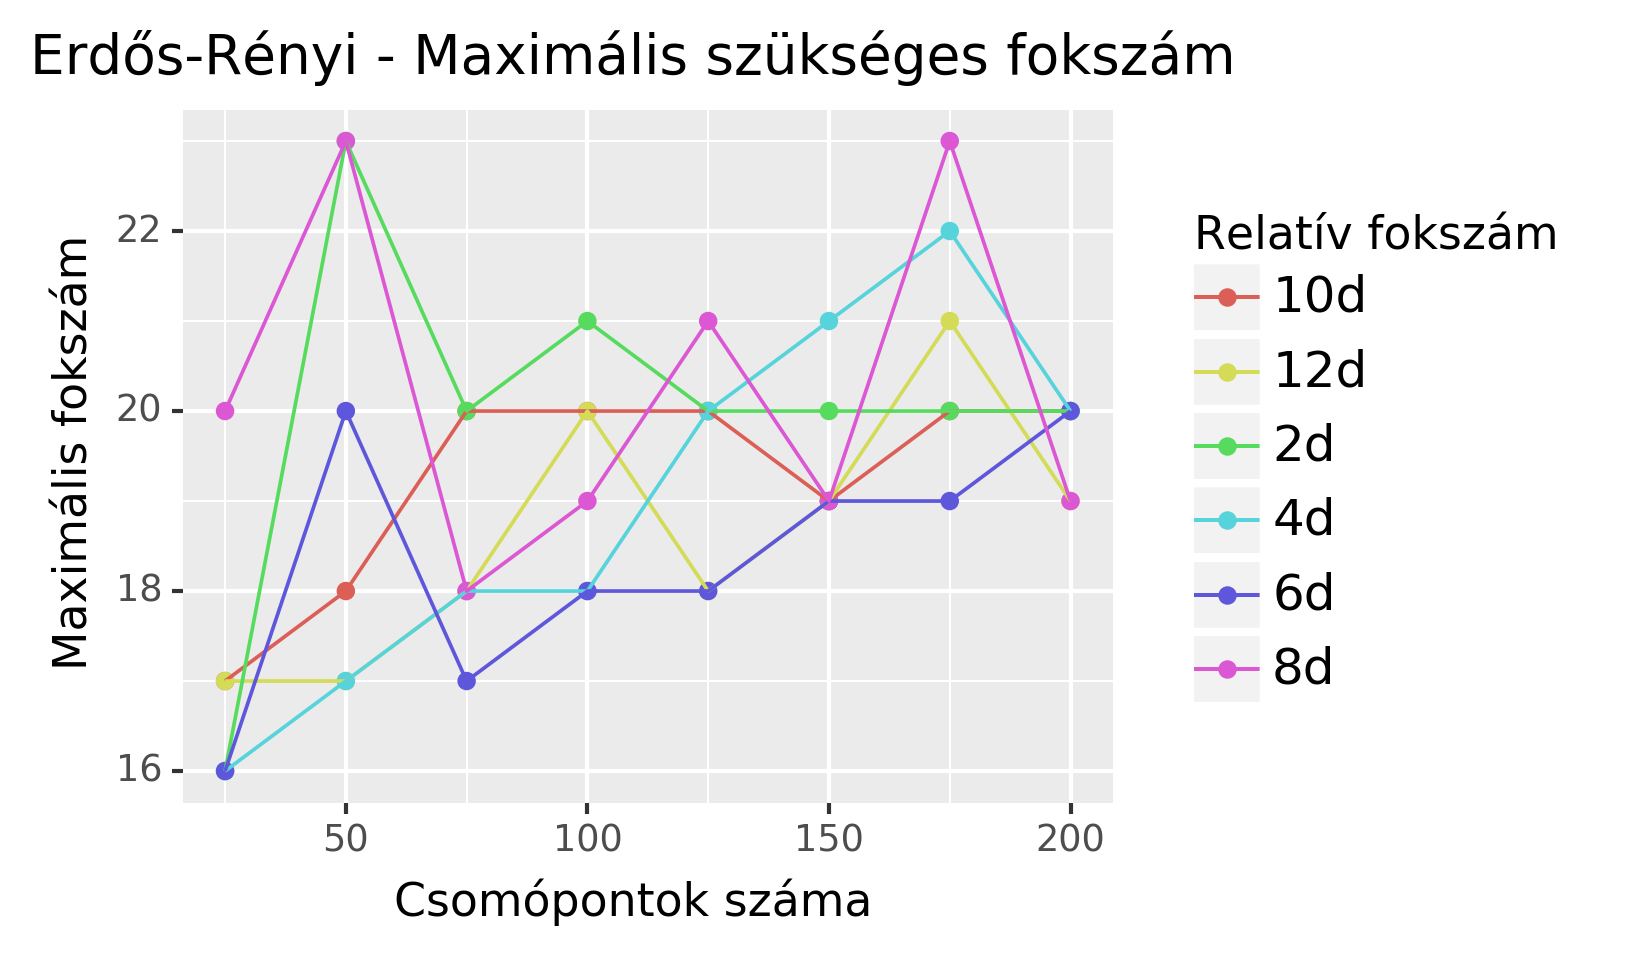
\includegraphics[width=0.49\linewidth]{pictures/delta_req.png}
		\caption{Erdős-Rényi gráf - Fa mennyiség összehasonlítás}
		\label{delta}
	\end{center}
\end{figure}

A következő szempont amiben változtak a gráfok, hogy mekkora terhelés legyen az éleken.
Itt két csoportba lehet sorolni a teszteket, ahol egytől tízig véletlenszerűen volt kiválasztva, a második esetben pedig minden él egységesen egy terhelést kapott.

Következő szempont amit figyelve volt az maga az algoritmus változtatása, hogy mennyi fa készüljön el, és hogy milyen stratégiával.

Végül pedig, hogy a mérési hiba minimalizálásának érdekében az fent említett paraméterek összes kombinációjára húsz teszt futott le. 
Összességében 384.000 teszt készült le, amit meg lehet találni a projekt GitHub oldalán.

\section{Metrikák}

Tesztelés során különböző metrikák kerültek rögzítésre, amit a következők:

\begin{itemize}
	\item \cmd{graph} - gráf típusa 
	\item \cmd{vertex num} - csúcsok száma a gráfban
	\item \cmd{constant} - a gráfhoz tartozó konstans paraméter 
	\item \cmd{congestion} - torlódás az eredeti értékekkel
	\item \cmd{real congestion} - a torlódás normalizálva egyre
	\item \cmd{avg route len} - átlag úthossz
	\item \cmd{delta} - fa $\Delta$ fokszáma
	\item \cmd{max delta} - a maximális $\Delta$ fokszám
	\item \cmd{dan} - a $\Delta$ megadott fokszám, ami lehet relatív is
	\item \cmd{most congested route} - a legnagyobb torlódással rendelkező él
	\item \cmd{max route len} - a maximális úthossz
	\item \cmd{avg tree weight} - az átlag fa súlya
	\item \cmd{most tree ratio} - a legnagyobb arány fa átlag ágsúlya és a legnehezebb ág között
	\item \cmd{tree count} - az épített fák száma
	\item \cmd{type} - a fa építései algoritmus típusa
	\item \cmd{start entropy} - a kezdeti költség mátrix entrópiája
\end{itemize}
	

\chapter{Teszt eredmények kiértékelése}

\section{Entrópia}

A különböző gráf típusok különböző entrópiával rendelkeznek.
Az entrópia diszkrét valószínűségi változóra felírható a következő képlettel\cite{DBLP:journals/corr/AvinMS17}:  

\[H(X) = \sum_{i=1}^{n} p(x_i) \cdot log_2\frac{1}{p(x_i)}; \; \forall i\in[1, ..., n] \land x_i = \sum_{1}^{n} demaind\_matix[i][n]\] 

Megjegyzés: mikor \(0\cdot log_2\frac{1}{0}\) értéket vesz fel az \(x_i\) változó, akkor legyen \(x_i=0\). 
Legyen \(\bar{p}\) a demand mátrix, ekkor \(H(\bar{p})\) megegyezik a következővel \(H(p_1, p_2, ..., p_n)\), ahol \(p_i\) egy sora a mátrixnak.
Ha teljesül, hogy \(p_i > 0\) és $\sum_{i}p_i = 1$ és a \(\bar{p}\) egyenletes eloszlást követ, akkor a véletlenszerű gráfban az entrópiára felső korlátja \(H(\bar{p}) = \log n\), ahol $n$ a csomópontok száma.

A fenti képlet segítségével ki lehet számolni az entrópiát a különböző véletlen szerűen készített gráfokra.
A következő grafikon mutatja, hogy a tesztek során használt véletlenszerű gráfoknak mennyi az entrópiájuk.
Eredmény a \ref{entropy} ábrán.

\begin{figure}[H]
	\begin{center}
		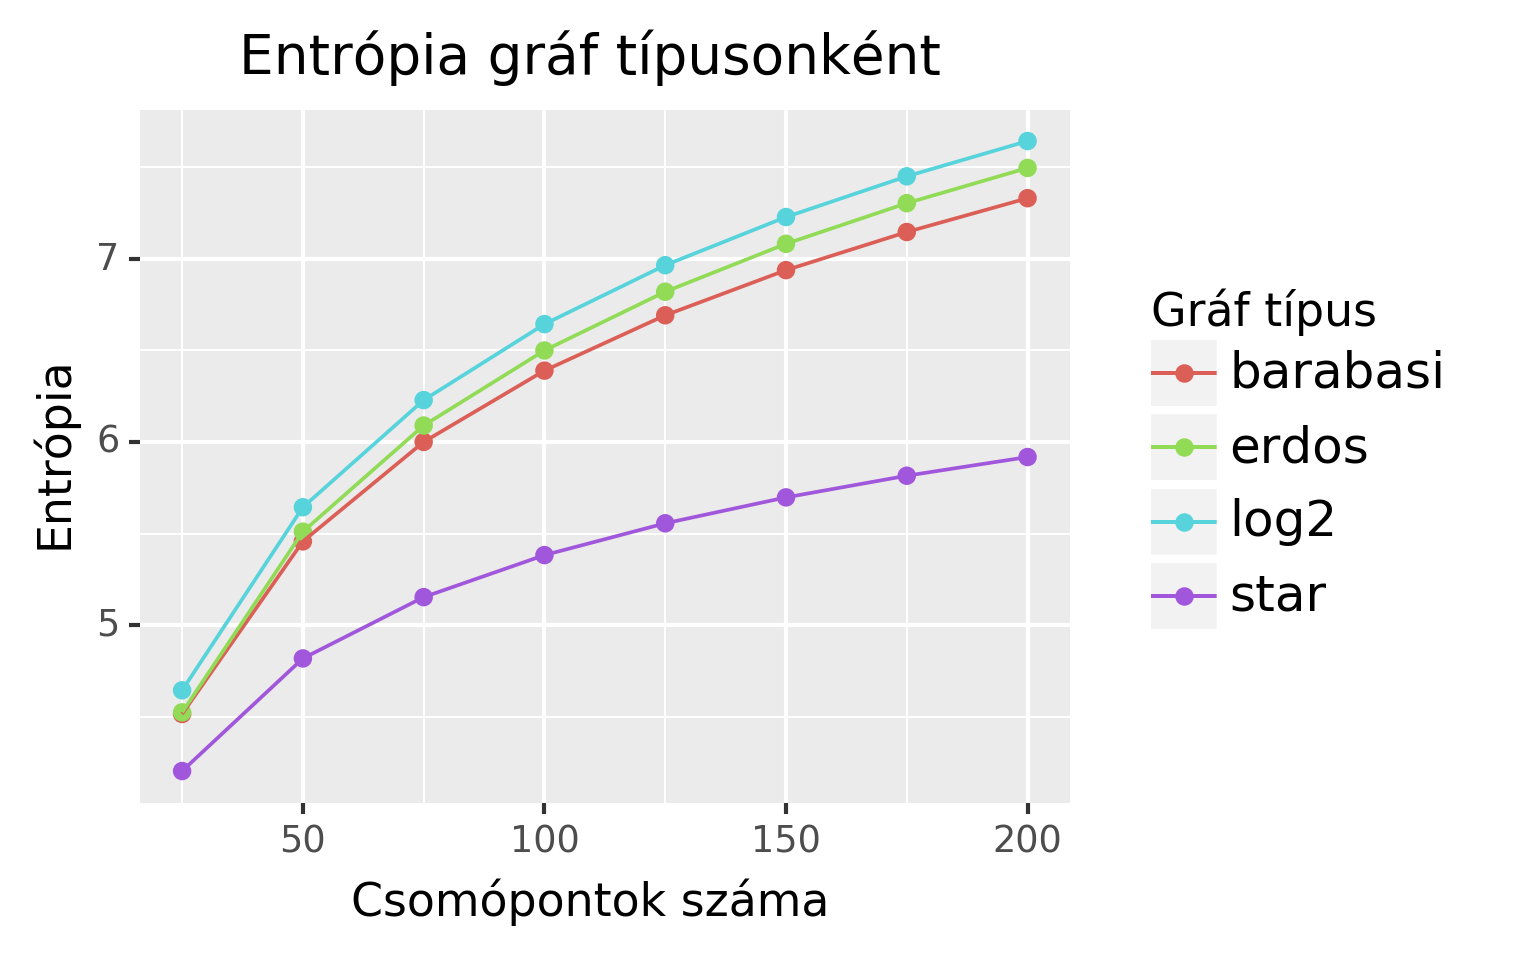
\includegraphics[width=0.9\linewidth]{pictures/entropy.png}
		\caption{Entrópia}
		\label{entropy}
	\end{center}
\end{figure}

A grafikonon látható, hogy az Erdős-Rényi gráfnak van a legnagyobb entrópiája, ami várható is volt, mivel ott egy valószínűség változó határozza meg mennyi éle lesz a gráfnak.
Ezt követi a Barabási-Albert gráf, ahol tudjuk mennyi élt várunk, annak függvényében mennyi régi csomópontra kell kapcsolódnia az új csomópontnak.
Majd végül a legkisebb entrópiát a csillag eredményez.
Ez várható is volt, mert az élek csúcsok csak a csillag középpontokhoz csatlakoznak, máshova nem.

\section{Úthossz}

\subsection{Általános eset}

A tesztek során a konstans érték határozta meg, hogy mennyire volt kitöltve a demand mátrix.
Ezért először nézzük meg mennyire van kihatással a mátrix kitöltöttsége az eredményekre.

Eredmény a \ref{density-len} ábrán.

\begin{figure}[H]
	\begin{center}
		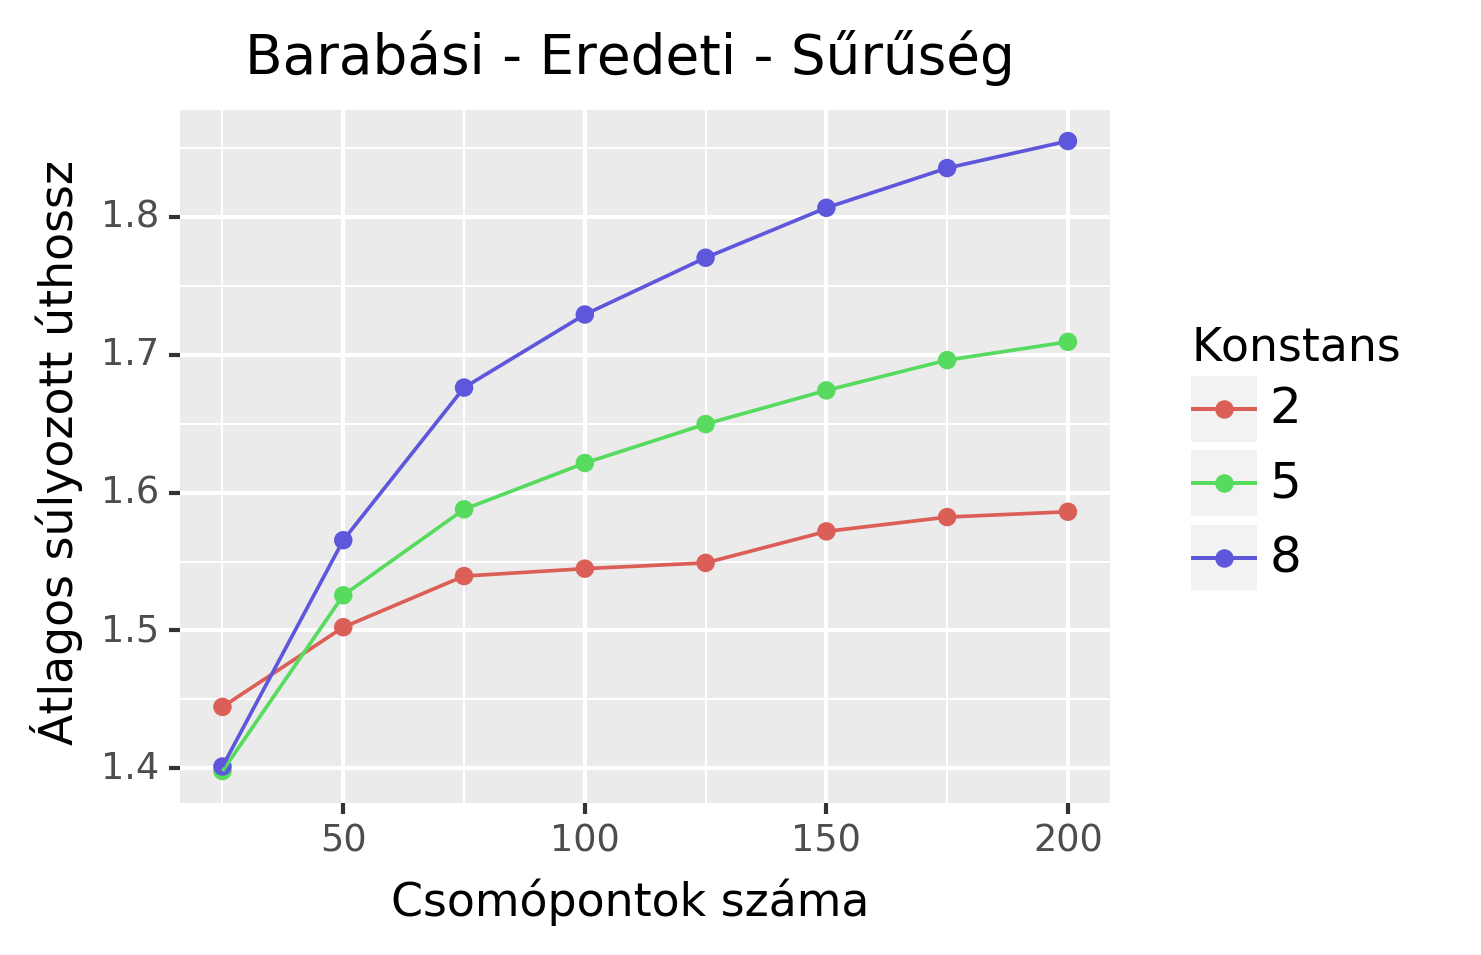
\includegraphics[width=0.9\linewidth]{pictures/density_len.png}
		\caption{Úthossz - Sűrűség}
		\label{density-len}
	\end{center}
\end{figure}

A grafikonon a Barabási-Albert gráf eredményei látható, az eredeti fa számosságával, azaz a fele-fele arányban elosztott, és a fák pedig az eredeti algoritmussal készültek el.
A hálózatban az összes szereplő él súlya 1, normalizálás után pedig
\(\frac{1}{|E|}\).
Mint látható a grafikonon, minél ritkább a mátrix, annál rövidebbek az úthosszak is.
Ezért a további grafikonoknál már csak a konstans 5 értékű eredményeket fogom vizsgálni, mivel az ad egy jó közelítést az átlagra.

\subsection{A fa építő algoritmusok összehasonlítása}

\subsubsection{Eredeti fa számosság}

Az általános esetben csak egy véletlenszerű gráf egy konkrét esetét néztük meg, most vizsgáljuk meg, hogy a különböző fa építési stratégiák, hogy befolyásolják az úthosszt.

Első véletlenszerű gráf típus a Barabási-Albert gráf, ahol az eredeti számosságú fát építjük. 
Eredmény a \ref{barabasi-len} ábrán.

\begin{figure}[H]
	\begin{center}
		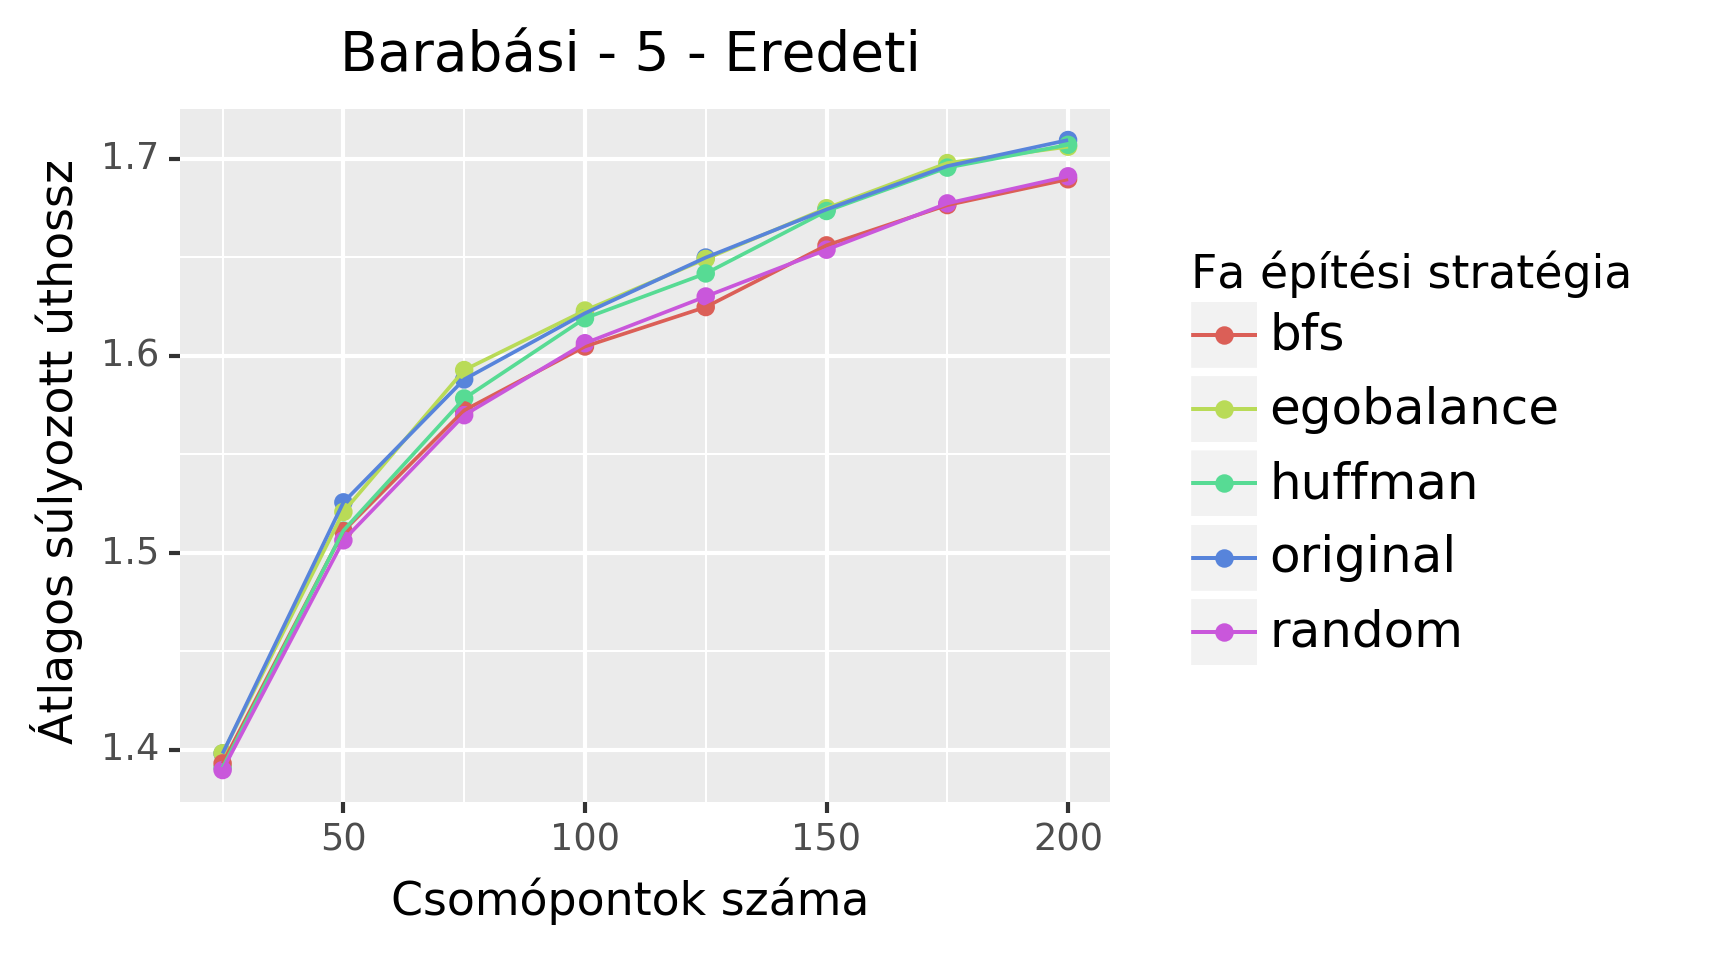
\includegraphics[width=0.9\linewidth]{pictures/barabasi_len_e.png}
		\caption{Barabási-Albert gráf - Úthossz}
		\label{barabasi-len}
	\end{center}
\end{figure}

A grafikonon látható, hogy három csoportba lehet besorolni az algoritmusokat. 
Az elsőbe tartozik az EgoBalance és az Eredeti algoritmus.
Ezek rendelkeznek a legnagyobb átlagos úthosszal és szinte ugyanazt az eredmény adják, mérési hiba különbséggel.
A következő a sorban a Huffman fa alapú algoritmus, ami kezdetben alacsonyabbról indul, de végül csatlakozik az első kettőhöz.
Legjobb két algoritmus pedig a Sorfolytonos fa és a Random fa.
Ez várható volt, mivel mindkettő ugyanazt az algoritmust használja, csak az értékekben különböznek.
Úthossz szempontjából ez a kettő adja mindig legkisebb fát, mivel egy teljes fát épít az algoritmus.


Következő véletlenszerű gráf típus amit vizsgálunk az az Erdős-Rényi gráf, itt is az eredeti számú fát építjük meg.
Eredmény a \ref{erdos-len} ábrán.

\begin{figure}[H]
	\begin{center}
		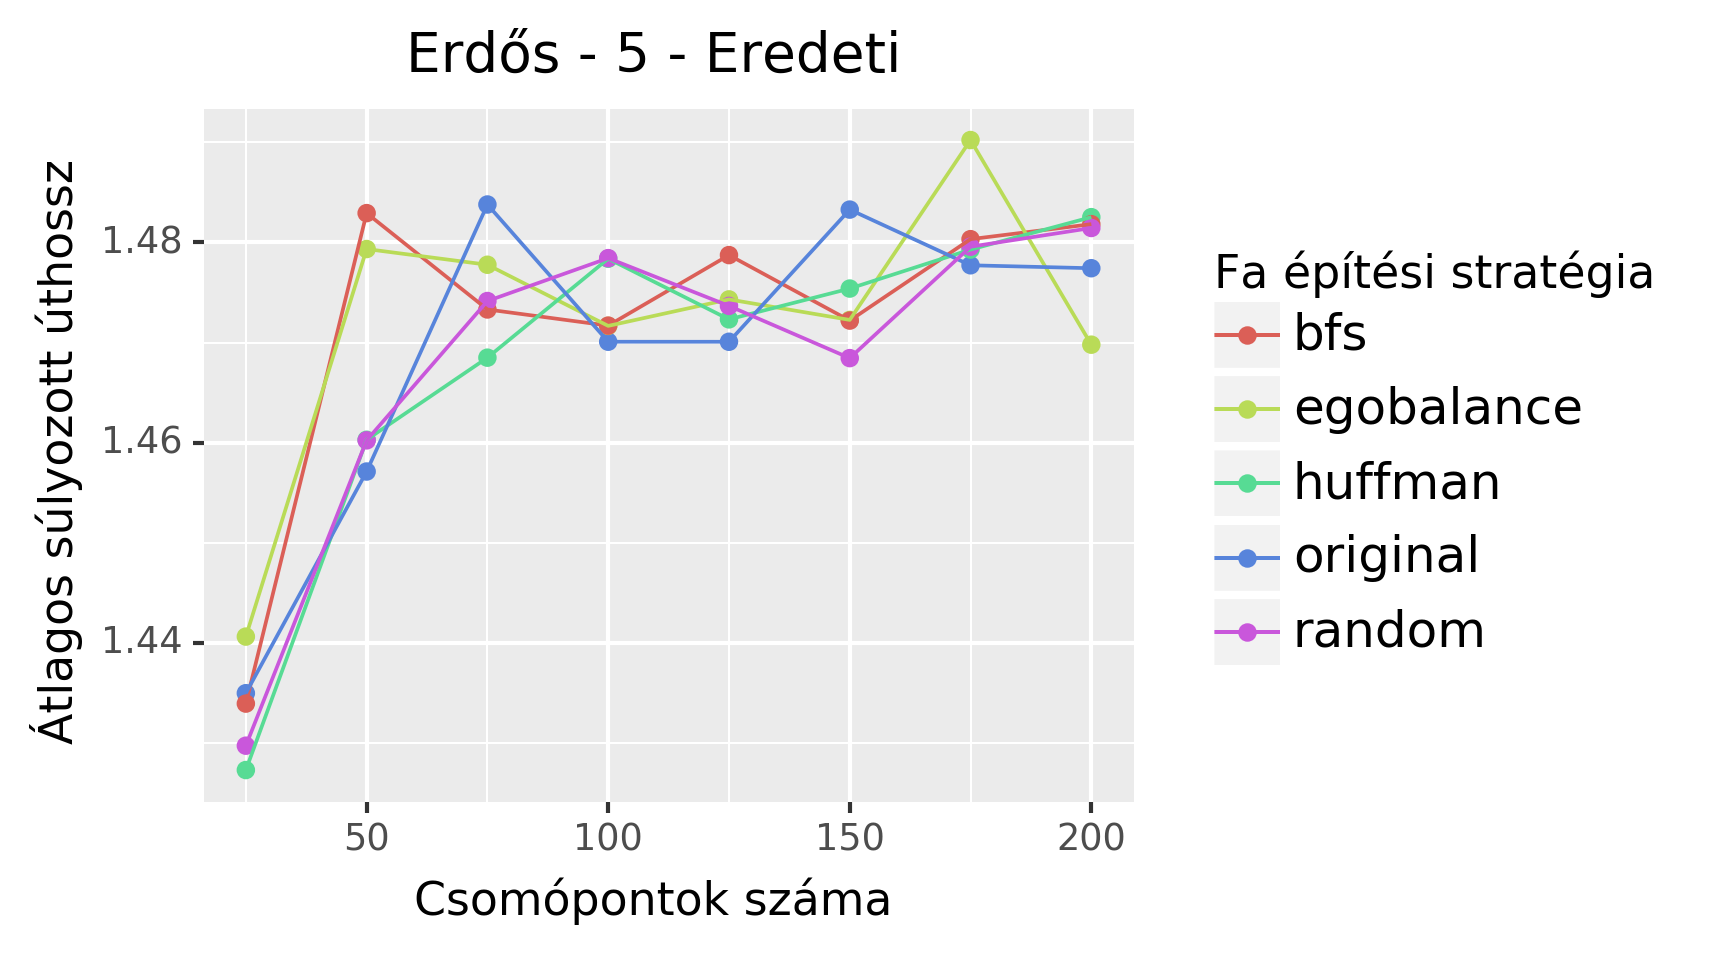
\includegraphics[width=0.9\linewidth]{pictures/erdos_len_e.png}
		\caption{Erdős-Rényi gráf - Úthossz}
		\label{erdos-len}
	\end{center}
\end{figure}

A grafikon itt már kicsit érdekesebb, mivel van egy kis oda-vissza mozgás az értékek közt. Azért látható hogy minden algoritmus hasonlóan eredményt eredményez.


Végül pedig nézzük meg a csillag gráfot az eredeti fa mennyiséggel a \ref{star-len} ábrán.

\begin{figure}[H]
	\begin{center}
		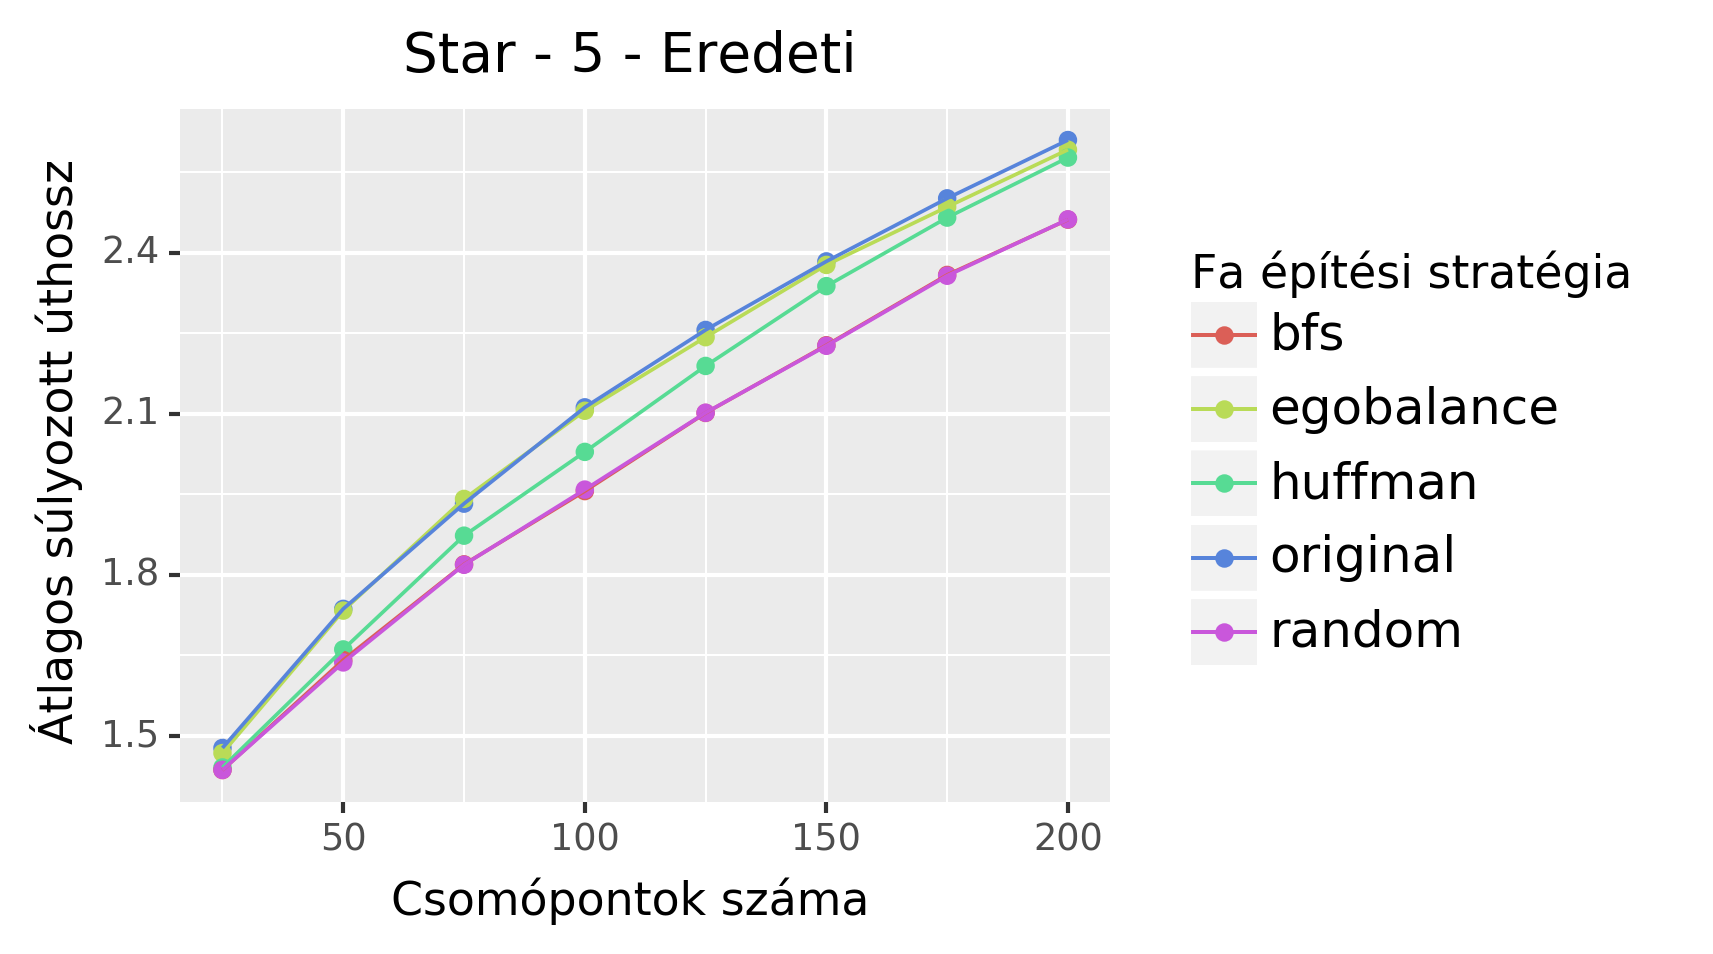
\includegraphics[width=0.9\linewidth]{pictures/star_len_e.png}
		\caption{Csillag gráf - Úthossz}
		\label{star-len}
	\end{center}
\end{figure}

Mint már láttuk a Barabási-Albert gráf esetében, itt is megvan a három egyértelmű kategória, ami teljesen megegyezik az előzővel.

\subsubsection{Módosított fa számosság}

Az előző részben láthattuk milyen eredményeket adnak az eredeti feltétel alapján a különböző algoritmusaink.
Most nézzük meg, hogyan változik az úthossz a fák számosságának függvényében. 
Azokat a fákat építjük meg amit ténylegesen nagyfokú, teljesül a magas fokszámú pontokra, hogy a fokszámuk legalább kétszerese az átlag fokszámnak.

Hasonlítsuk össze a Barabási-Albert gráf eredményeit a \ref{barabasi-tree-difference-len} ábrán.

\begin{figure}[H]
	\begin{center}
		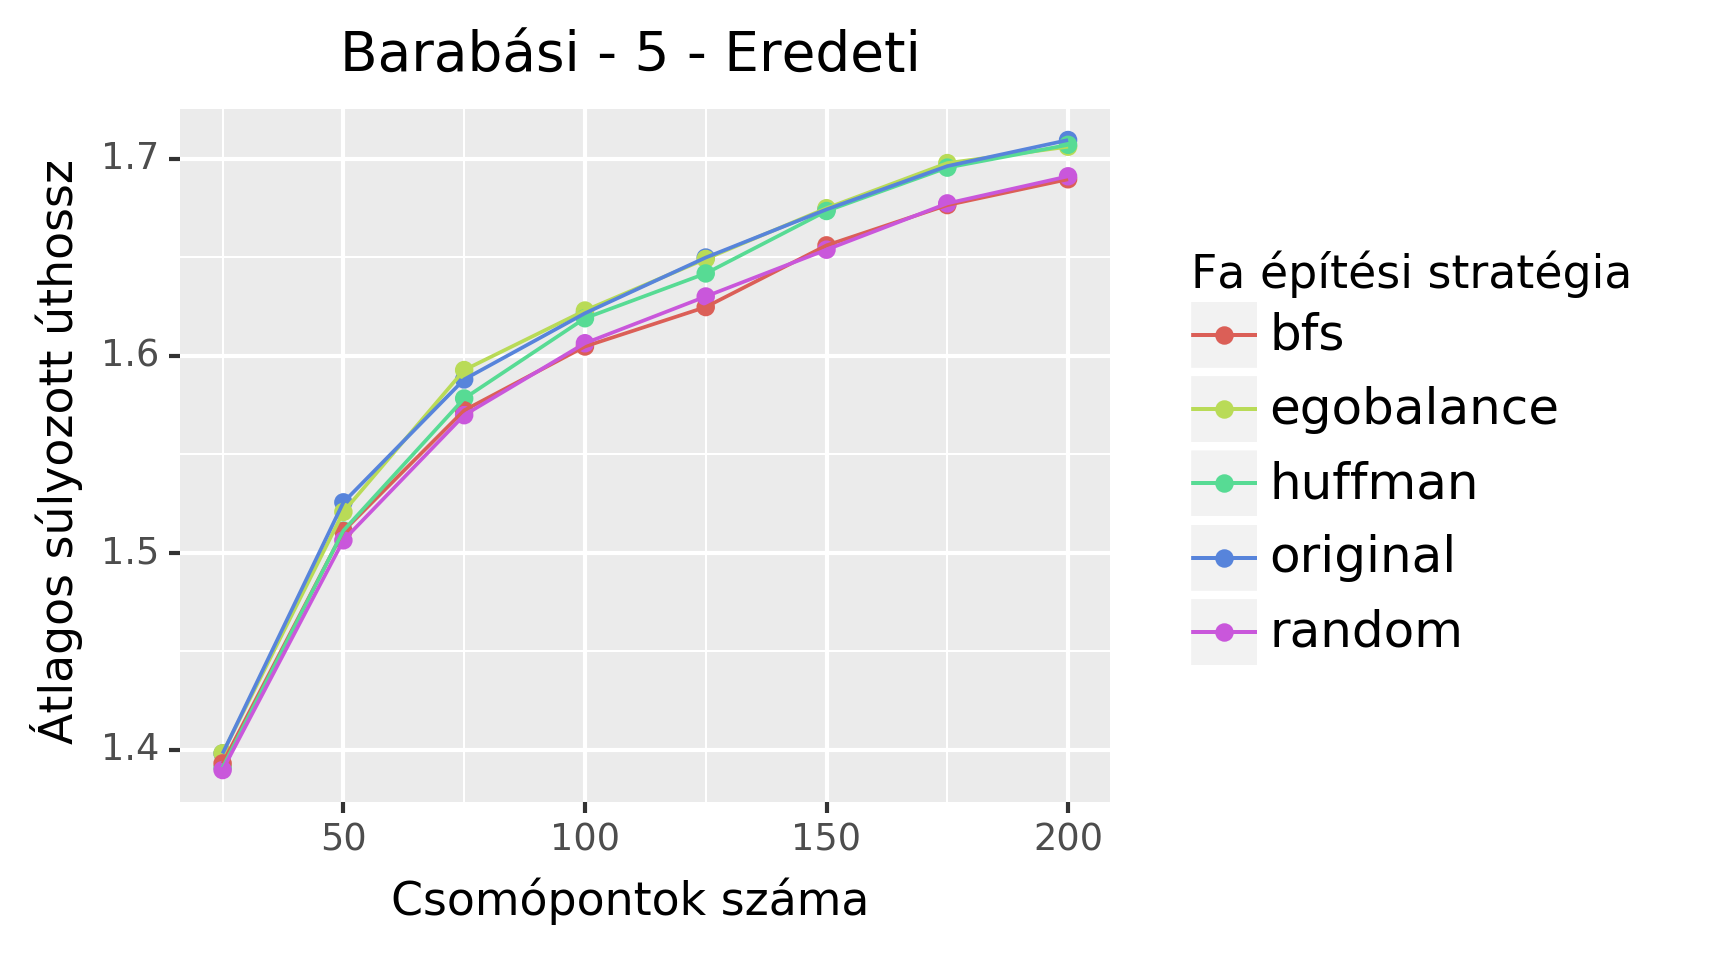
\includegraphics[width=0.49\linewidth]{pictures/barabasi_len_e.png}
		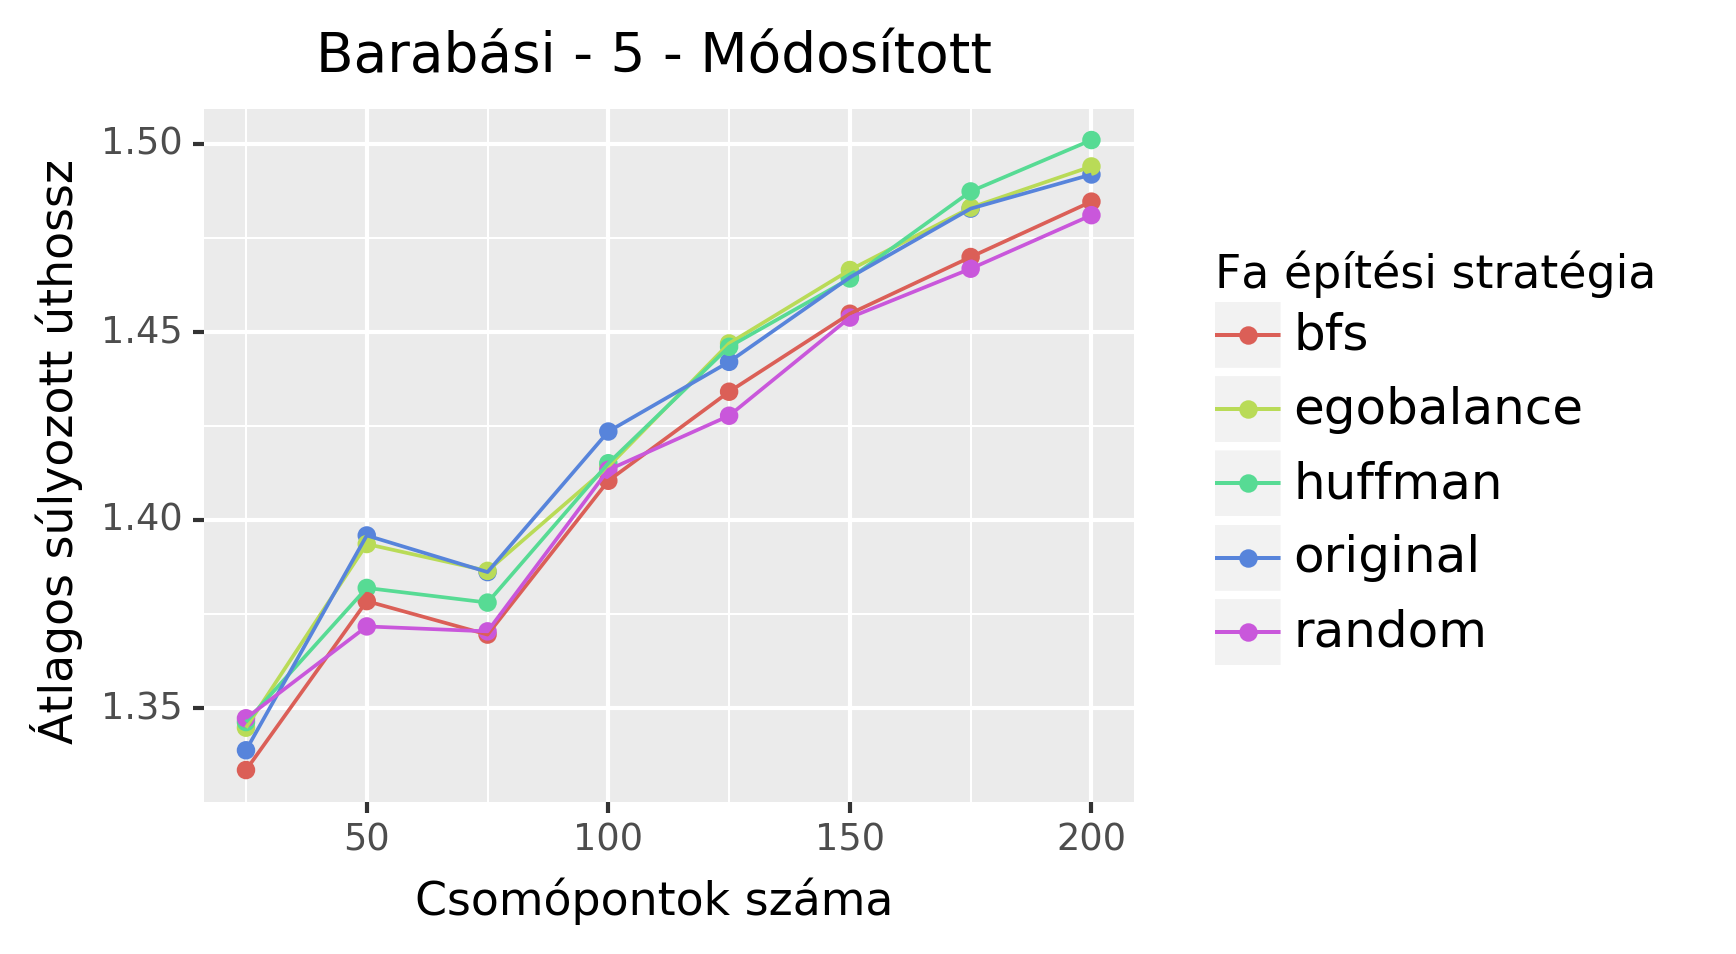
\includegraphics[width=0.49\linewidth]{pictures/barabasi_len_m.png}
		\caption{Barabási-Albert gráf - Fa számosság összehasonlítás}
		\label{barabasi-tree-difference-len}
	\end{center}
\end{figure}

Első jelentős különbség, hogy csökken az átlag úthossz.
Az gráf iránya továbbra is tartja az eredeti trendjét, egy kis beeséssel a 75 csúcsú gráfnál, de látható, hogy javít a módosítás az eredeti algoritmushoz képest.

Következő gráfunk az Erdős-Rényi gráf a \ref{erdos-tree-difference-len} ábrán.

\begin{figure}[H]
	\begin{center}
		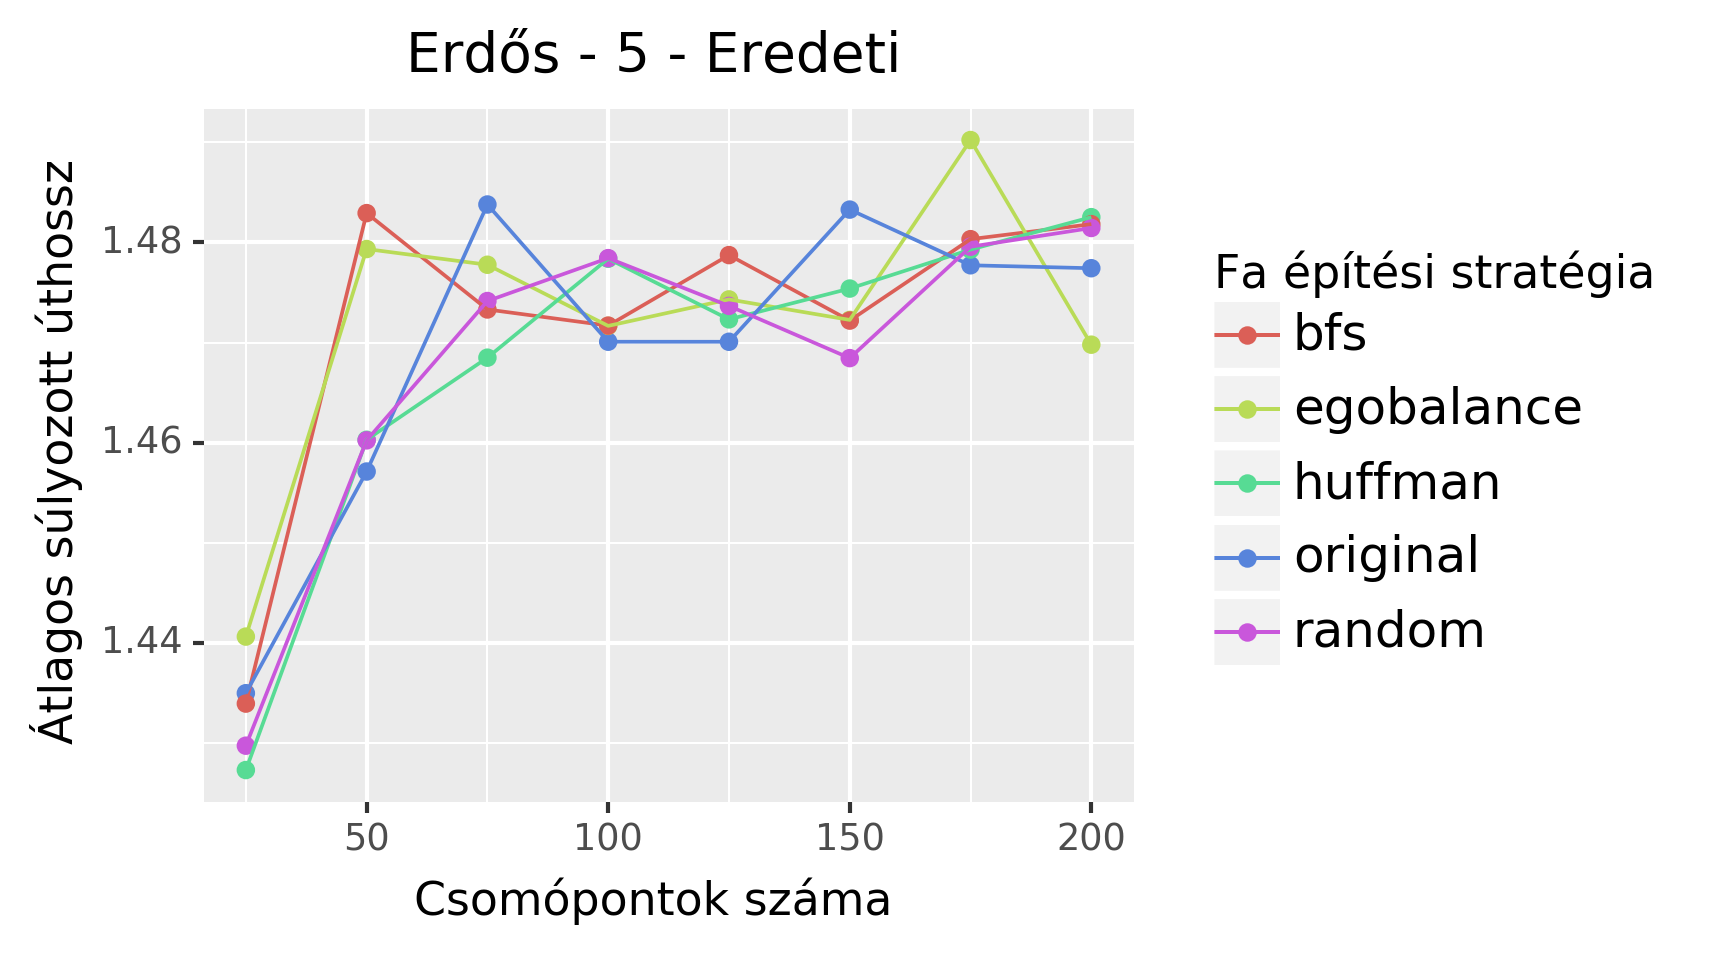
\includegraphics[width=0.49\linewidth]{pictures/erdos_len_e.png}
		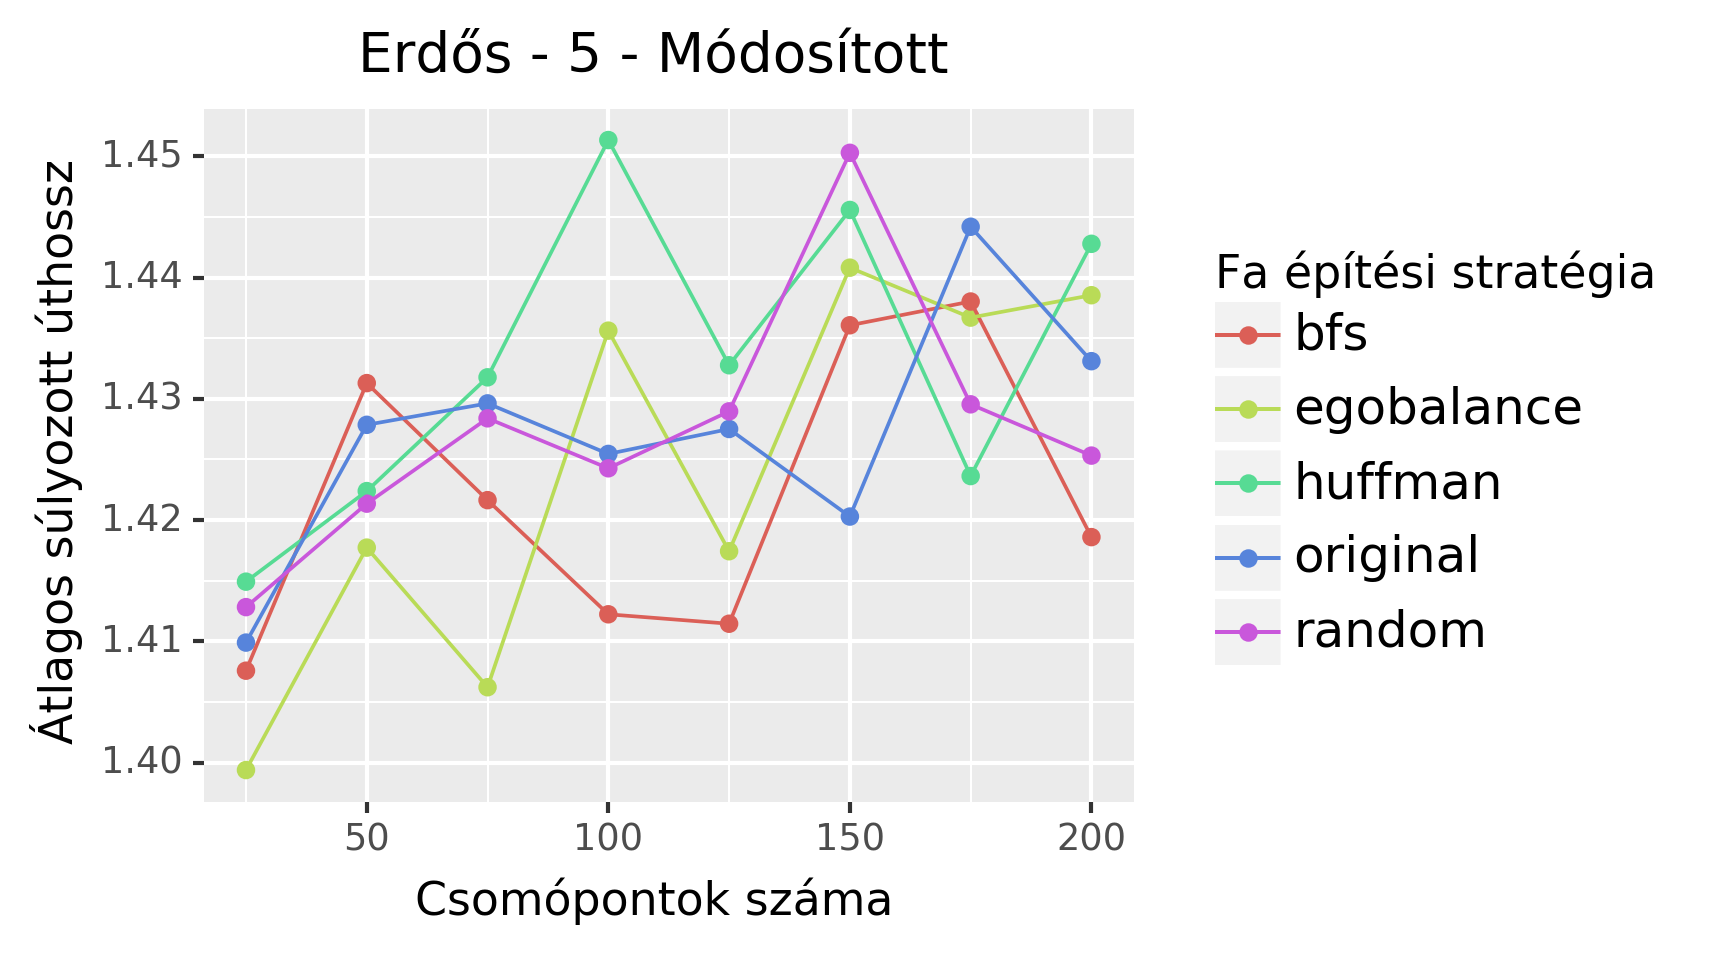
\includegraphics[width=0.49\linewidth]{pictures/erdos_len_m.png}
		\caption{Erdős-Rényi gráf - Fa számosság összehasonlítás}
		\label{erdos-tree-difference-len}
	\end{center}
\end{figure}

Amint látható, a gráf pontjai ingadoznak, ám ha hasonlítjuk az eredeti eredményekhez akkor tudunk következtetést levonni.
Az eredetihez képest az értékek kisebbek, ami a célunk volt a módosítás bevezetésével.

Végül nézzük meg a csillag gráfot a \ref{star-tree-difference-len} ábrán. 

\begin{figure}[H]
	\begin{center}
		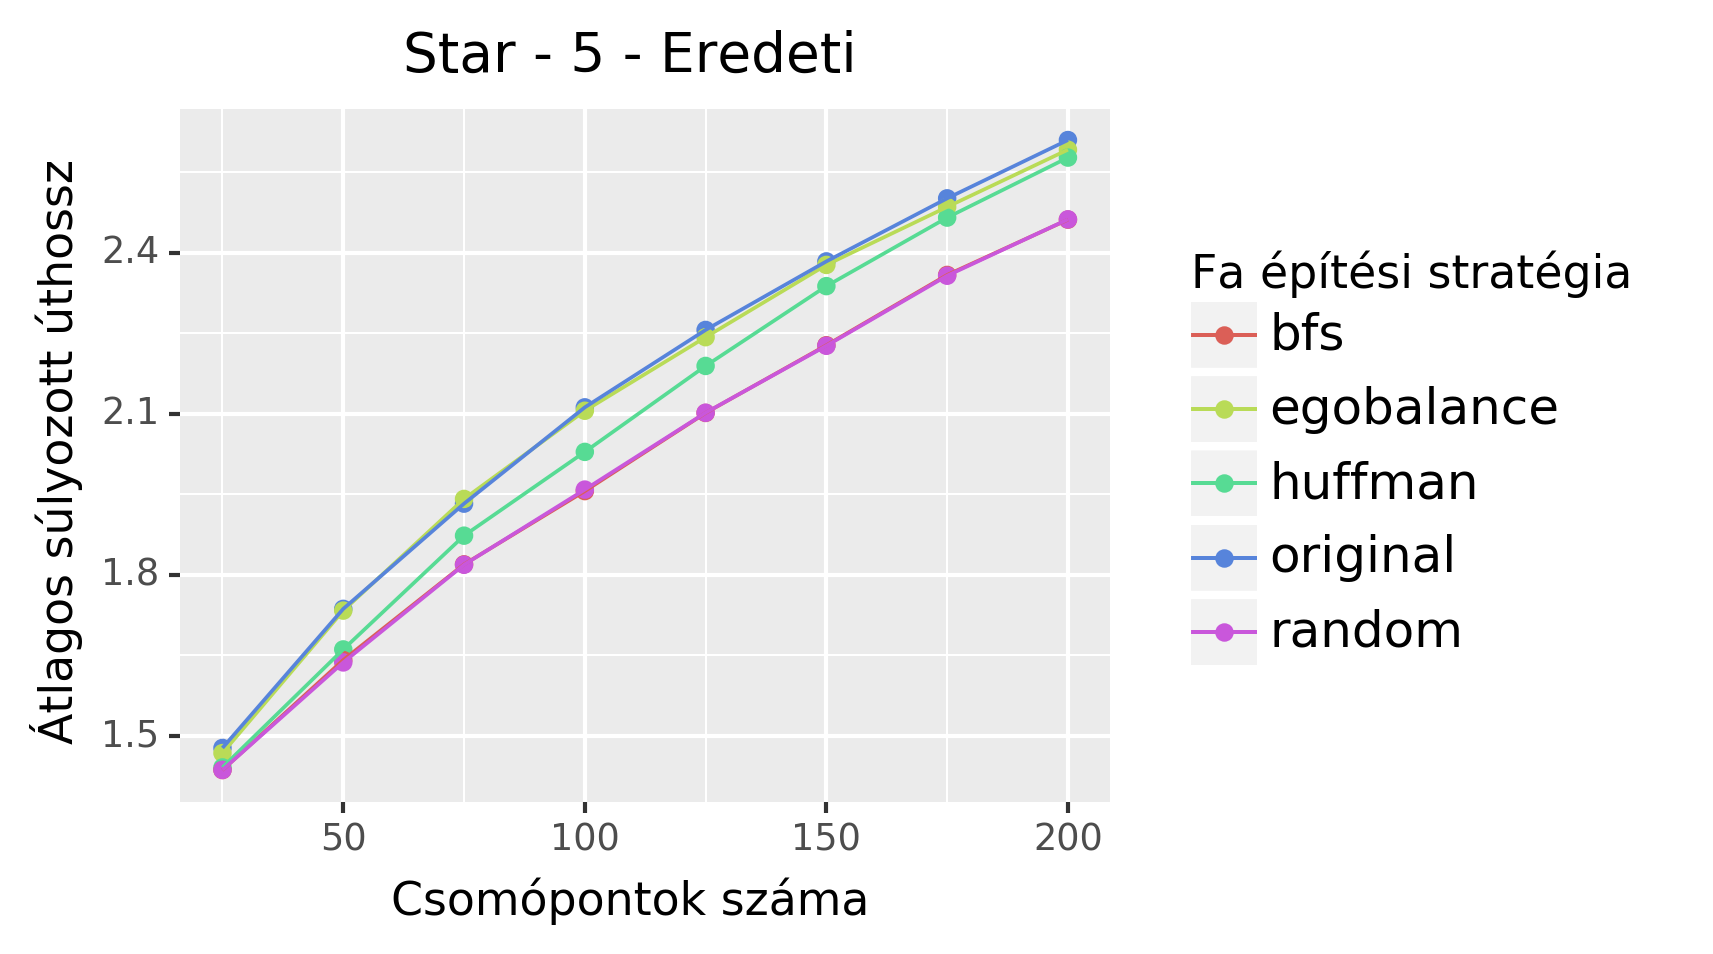
\includegraphics[width=0.49\linewidth]{pictures/star_len_e.png}
		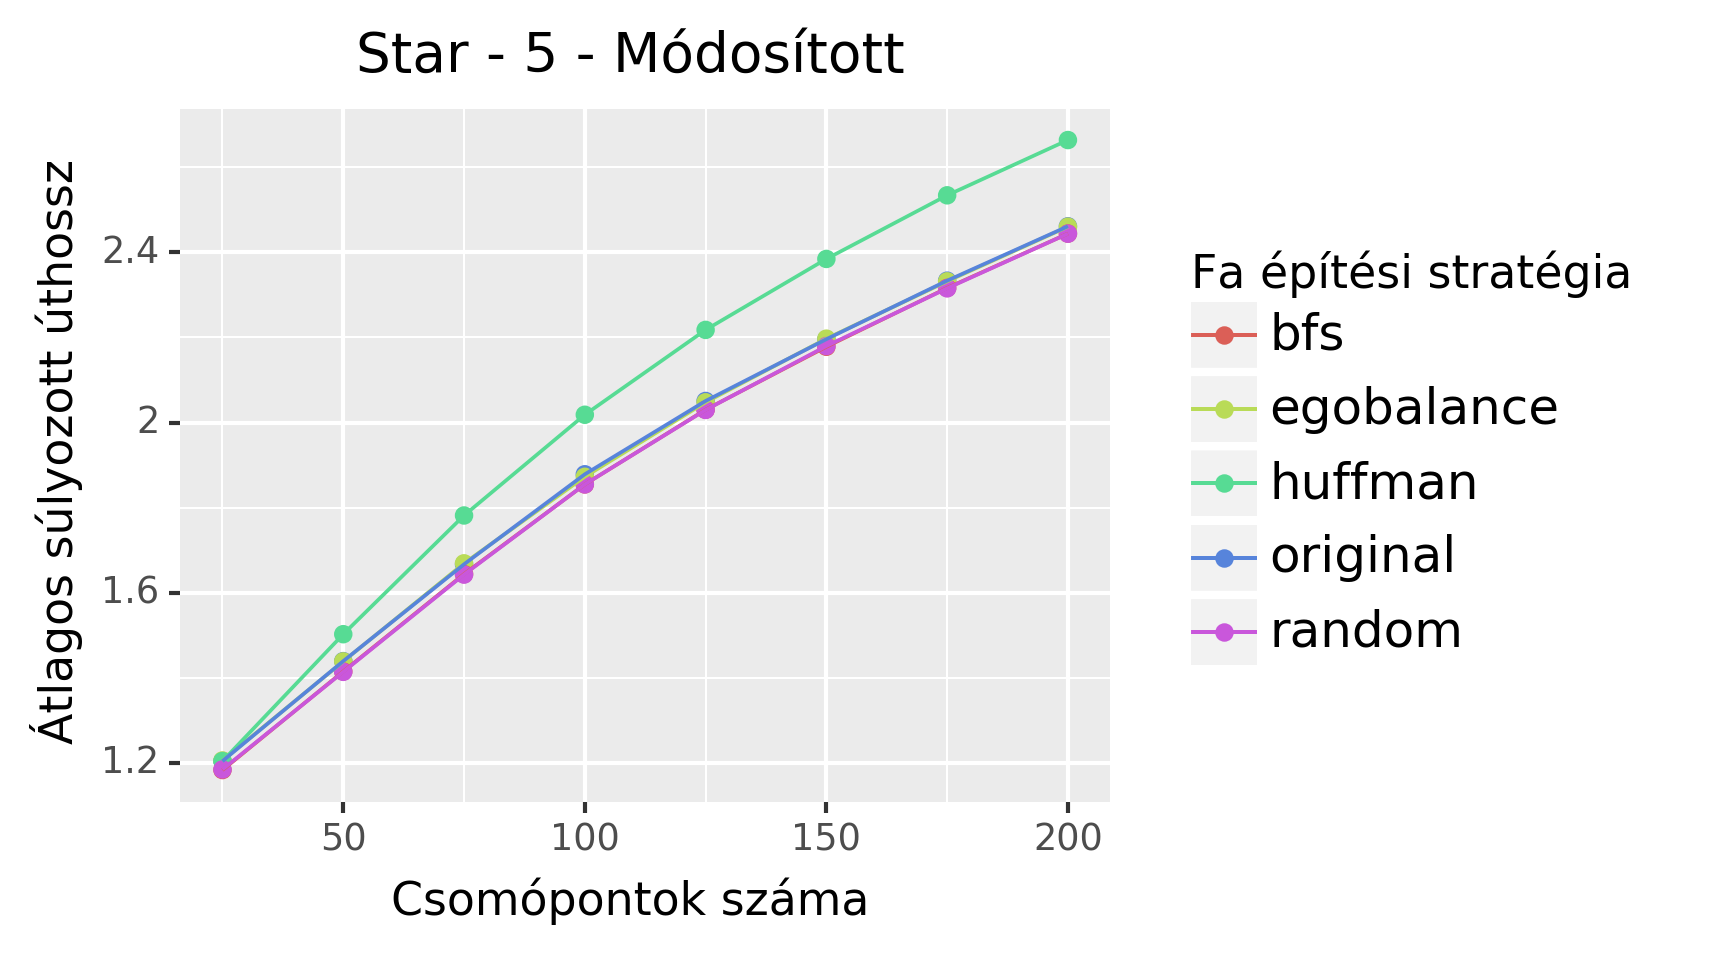
\includegraphics[width=0.49\linewidth]{pictures/star_len_m.png}
		\caption{Csillag gráf - Fa számosság összehasonlítás}
		\label{star-tree-difference-len}
	\end{center}
\end{figure}

Itt történt egy fordulat a grafikonon, először is amíg a Huffman fa alapú stratégia a közép értéket adta a két másik csoport között, itt most jelentősen rosszabb eredmény produkált.
A másik négy algoritmus meg javult az úthosszara nézve és megmaradt a relatív pozíciójuk.

\section{Torlódás}

\subsection{Általános eset}

Az úthosszhoz hasonlóan először nézzük meg, hogy az eredeti algoritmus milyen eredményt ad, attól függően mennyire sűrű a gráf.
Eredmény a \ref{density-con} ábrán.

\begin{figure}[H]
	\begin{center}
		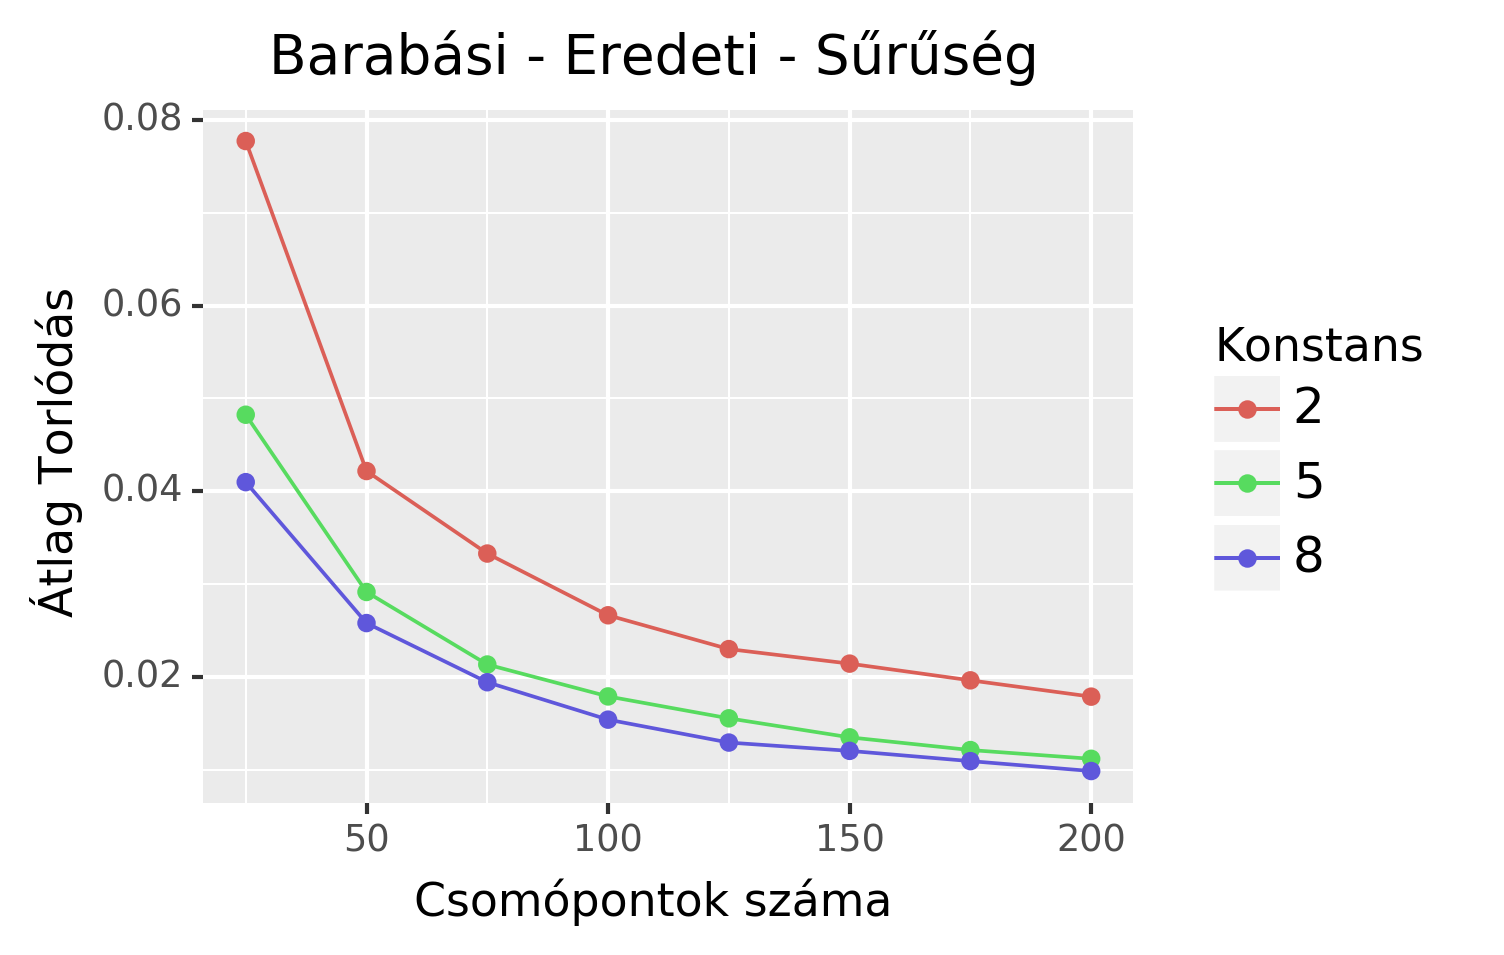
\includegraphics[width=0.9\linewidth]{pictures/density_con.png}
		\caption{Torlódás - Sűrűség}
		\label{density-con}
	\end{center}
\end{figure}

A grafikonon a Barabási-Albert gráf eredményei látható, az eredeti fa mennyiséggel és a fák pedig az eredeti algoritmussal készültek el.
A hálózatban az összes szereplő él súlya 1.
Mint látható a grafikonon, minél ritkább a mátrix, annál nagyobb a torlódás. 
Egy fontos észrevétel a két metrika között, még az úthossz átlagosan az egész mátrixra nézve adta meg az eredményt, addig a torlódás az egyértelműen a legnagyobb torlódás az útválasztási sémán.
Ezért ha kevés éllel rendelkezik a gráf, annál kevesebb lehetősége van olyan élt választani az algoritmusnak, ahol még alacsony a torlódás.
A további grafikonoknál már csak a konstans 5 értékű eredményeket fogom vizsgálni, mivel az ad egy jó közelítést az átlagos torlódása.

\subsection{A fa építő algoritmusok összehasonlítása}

\subsubsection{Eredeti fa számosság}

Az általános eset után, most vizsgáljuk meg, hogy a különböző fa építési stratégiák, hogy befolyásolják a torlódást.

Első véletlenszerű gráf ismét a Barabási-Albert gráf, ahol az eredeti mennyiségű fát építjük. Eredmény a \ref{barabasi-con} ábrán.

\begin{figure}[H]
	\begin{center}
		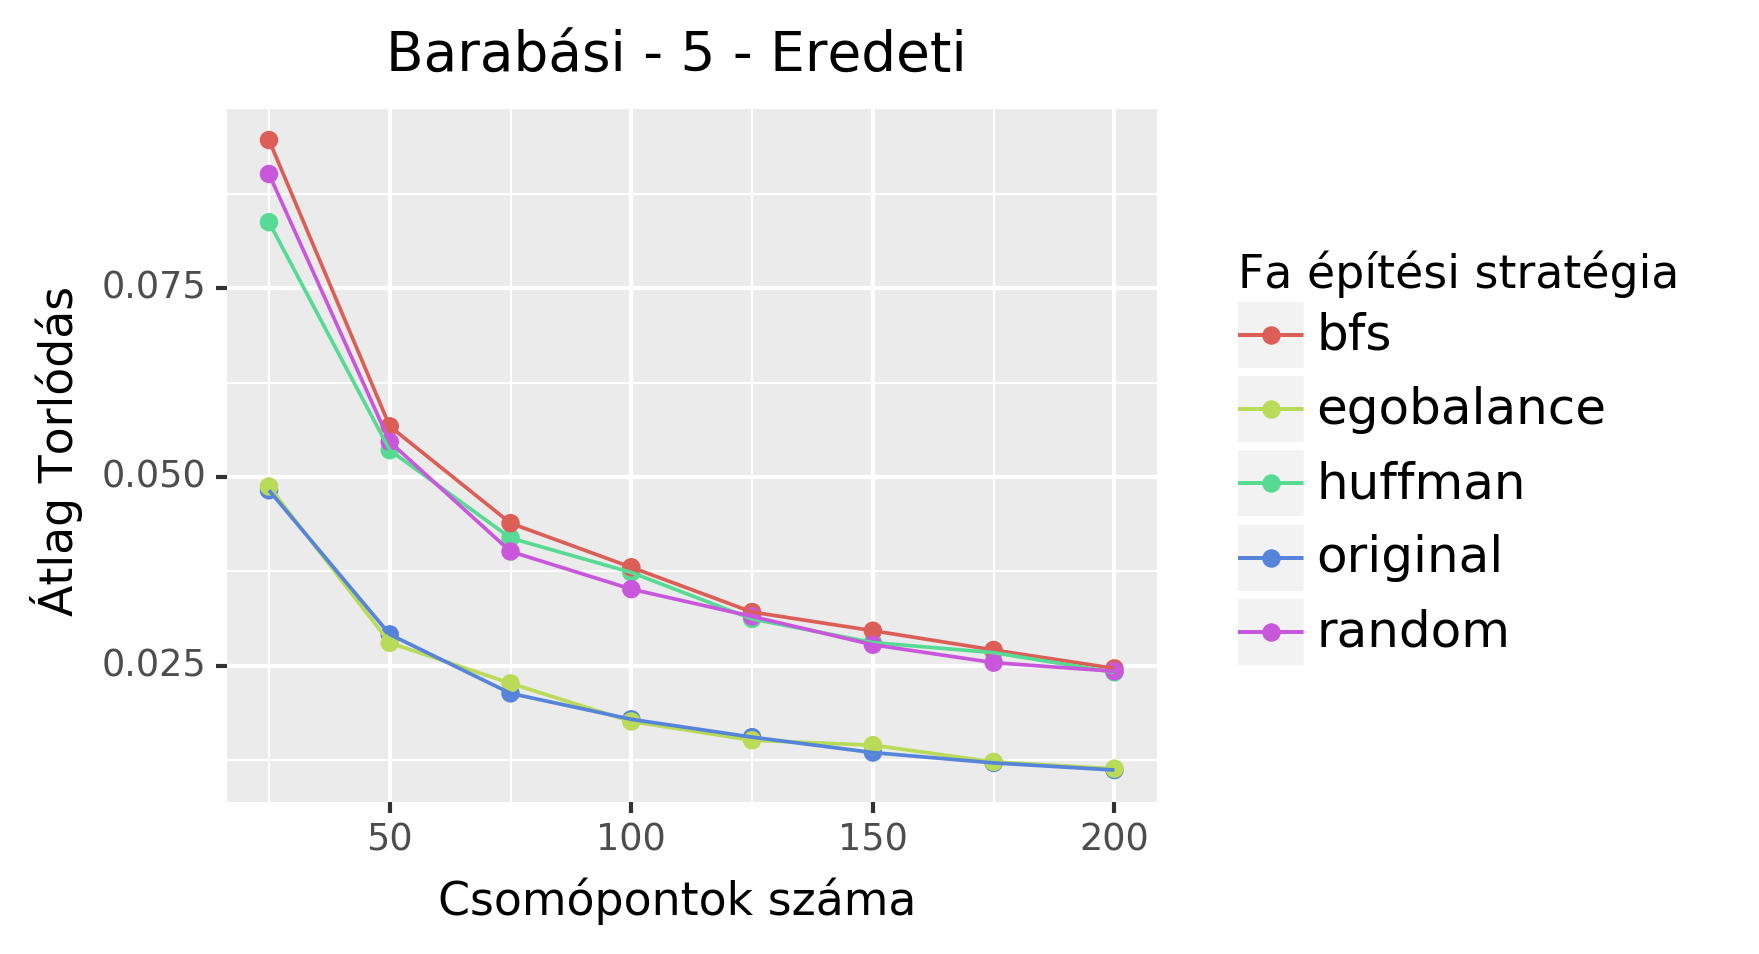
\includegraphics[width=0.9\linewidth]{pictures/barabasi_con_e.png}
		\caption{Barabási-Albert gráf - Torlódás}
		\label{barabasi-con}
	\end{center}
\end{figure}

A grafikonon látható, hogy két csoportba lehet besorolni az algoritmusokat. 
Az elsőbe tartozik az EgoBalance és az Eredeti algoritmus.
Ezek adják a legjobb eredményt és szinte azonosak.
A másik csoportba tartozik a maradék három algoritmus, a Sorfolytonos-, a Random- és a Huffman fa.
Itt egyértelmű miért jött ki ez az eredmény, mivel ez a három algoritmus egyáltalán nem veszi figyelembe a tényezőt, hogy mekkora a torlódás.

Következő véletlenszerű gráf típus az Erdős-Rényi gráf, itt is az eredeti számú fát építjük meg. 
Eredmény a \ref{erdos-con} ábrán.

\begin{figure}[H]
	\begin{center}
		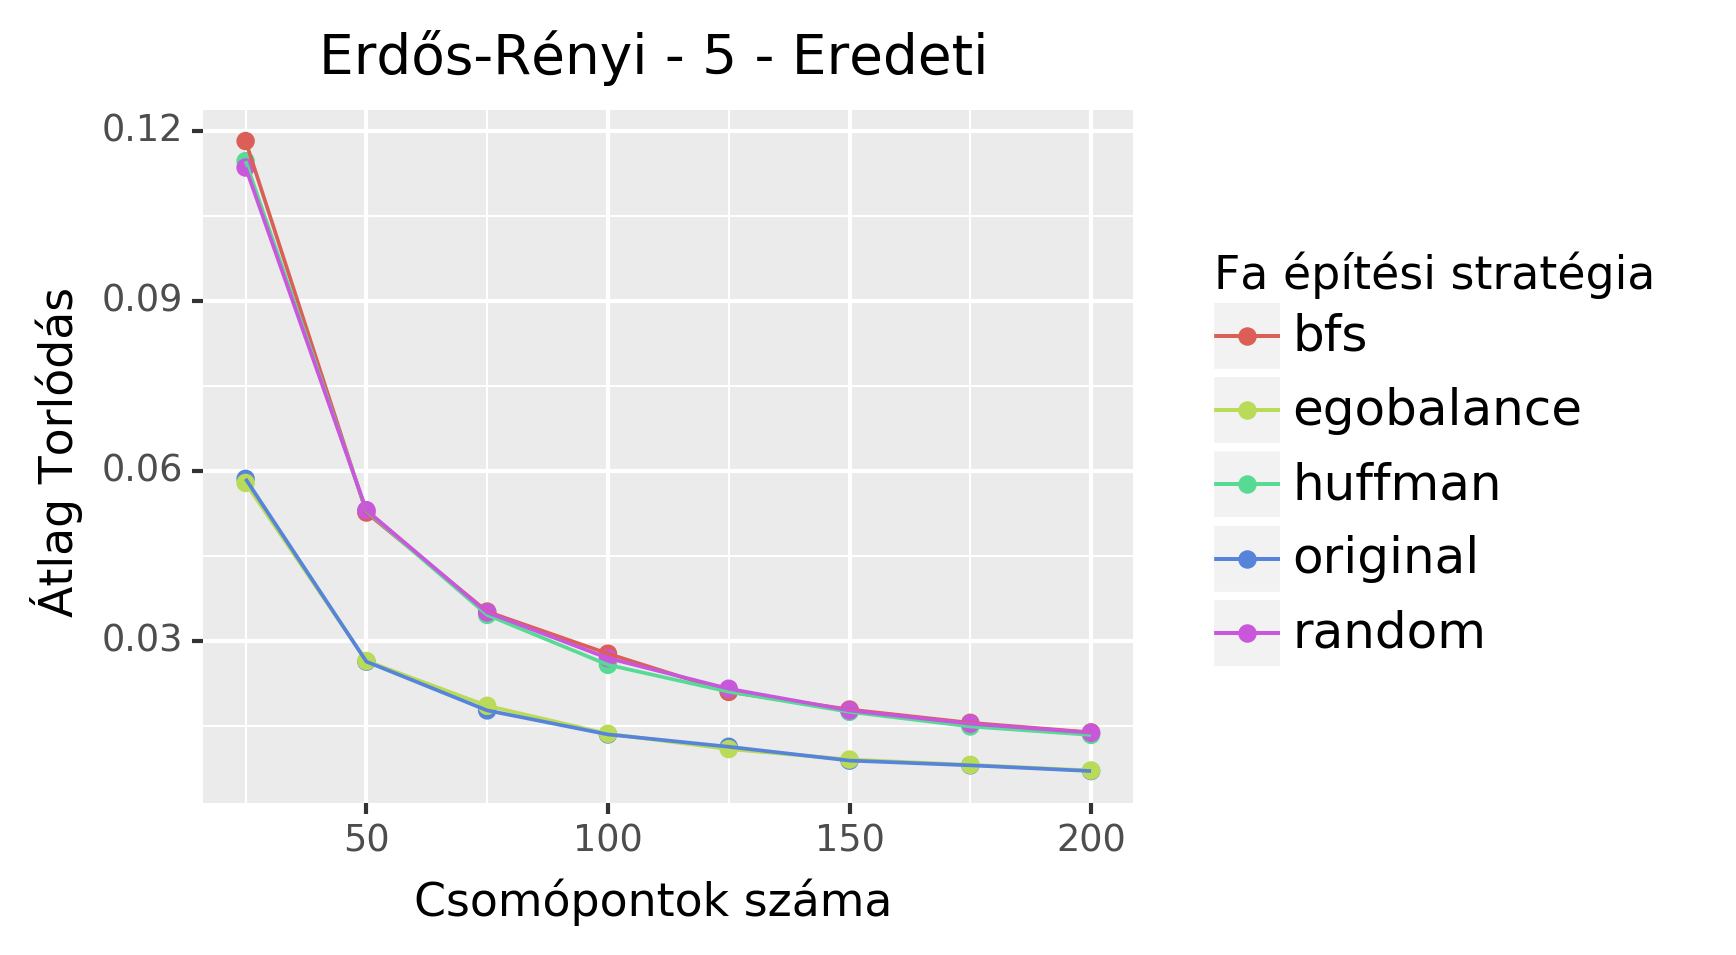
\includegraphics[width=0.9\linewidth]{pictures/erdos_con_e.png}
		\caption{Erdős-Rényi gráf - Torlódás}
		\label{erdos-con}
	\end{center}
\end{figure}

A grafikon szinte megegyezően ugyanazt az eredmény mutatja mint a Barabási-Albert gráf esetén.
Két csoport, ahol még mindig az Eredeti és az EgoBalance teljesítenek a legjobban.

Végül pedig nézzük meg a csillag gráfot az eredeti fa mennyiséggel a \ref{star-con} ábrán.

\begin{figure}[H]
	\begin{center}
		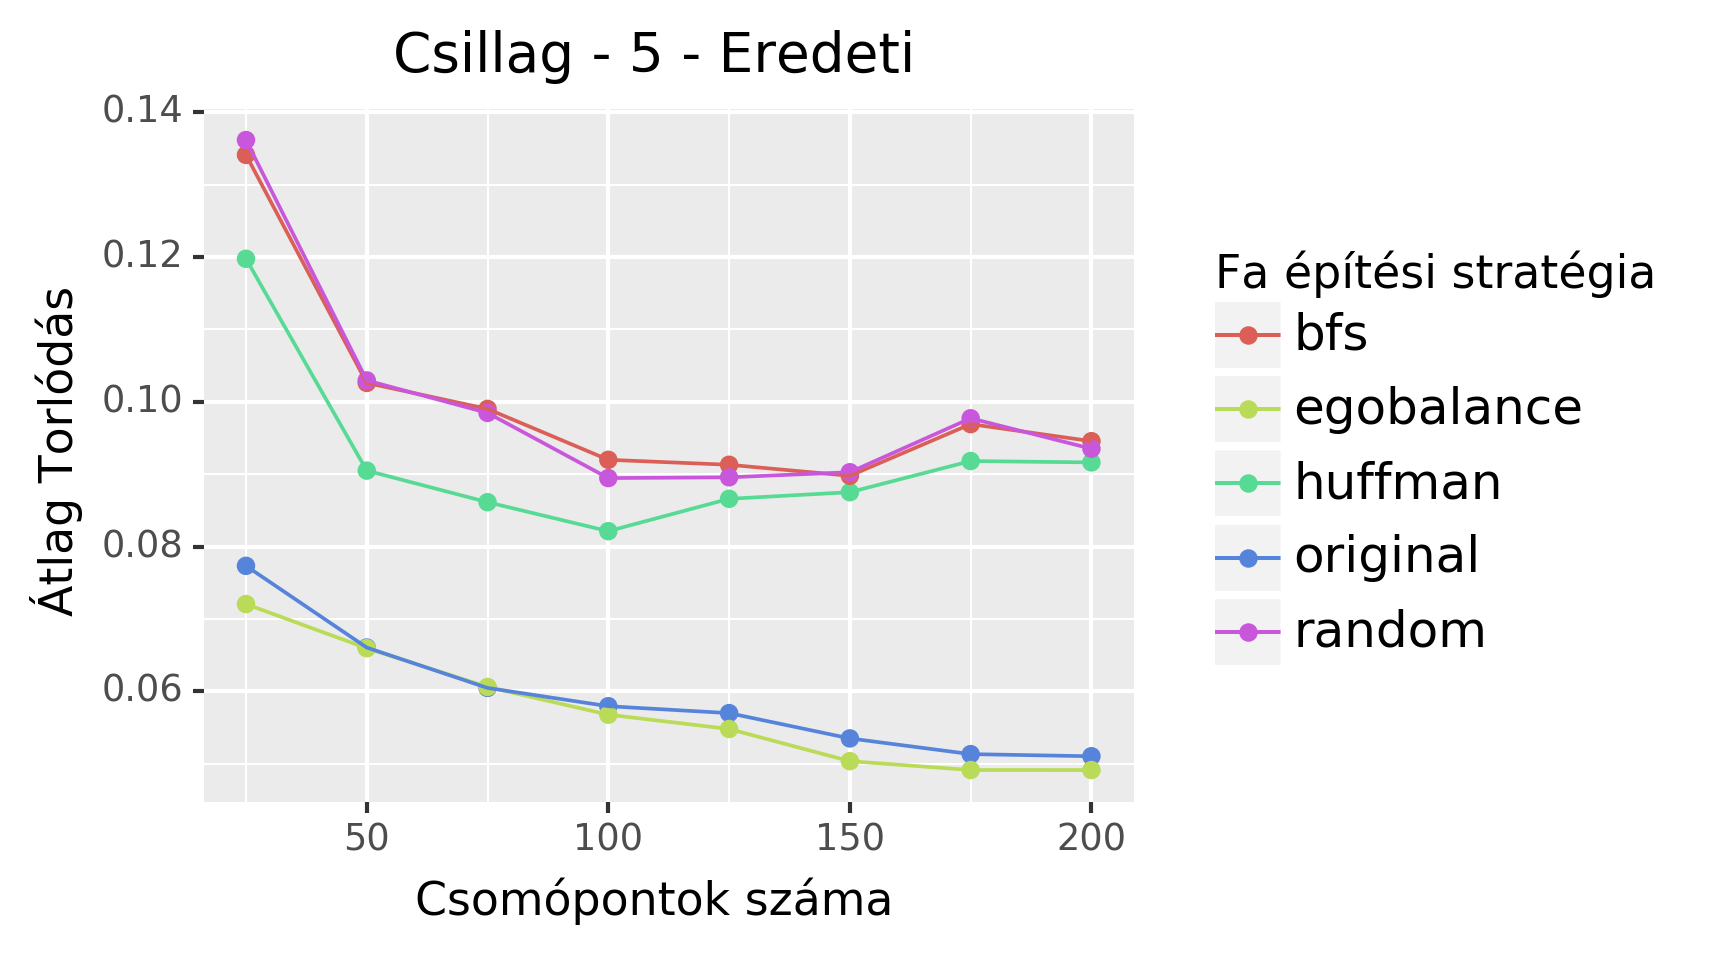
\includegraphics[width=0.9\linewidth]{pictures/star_con_e.png}
		\caption{Csillag gráf - Torlódás}
		\label{star-con}
	\end{center}
\end{figure}

Itt már elhatárolódik a Huffman fa a Sorfolytonos és Random fáktól, de nem eléggé, hogy megközelítse az Eredetit vagy az EgoBalance-ot.

\subsubsection{Módosított fa számosság}

Az előző részben láthattuk milyen eredményeket adnak az eredeti feltétel alapján a különböző algoritmusaink.
Most nézzük meg, ha változik a torlódás a fák számosságának függvényében. 
Azokat a fákat építjük meg amit ténylegesen nagyfokúak.

Hasonlítsuk össze a Barabási-Albert gráf eredményeit a \ref{barabasi-tree-difference-con} ábrán.

\begin{figure}[H]
	\begin{center}
		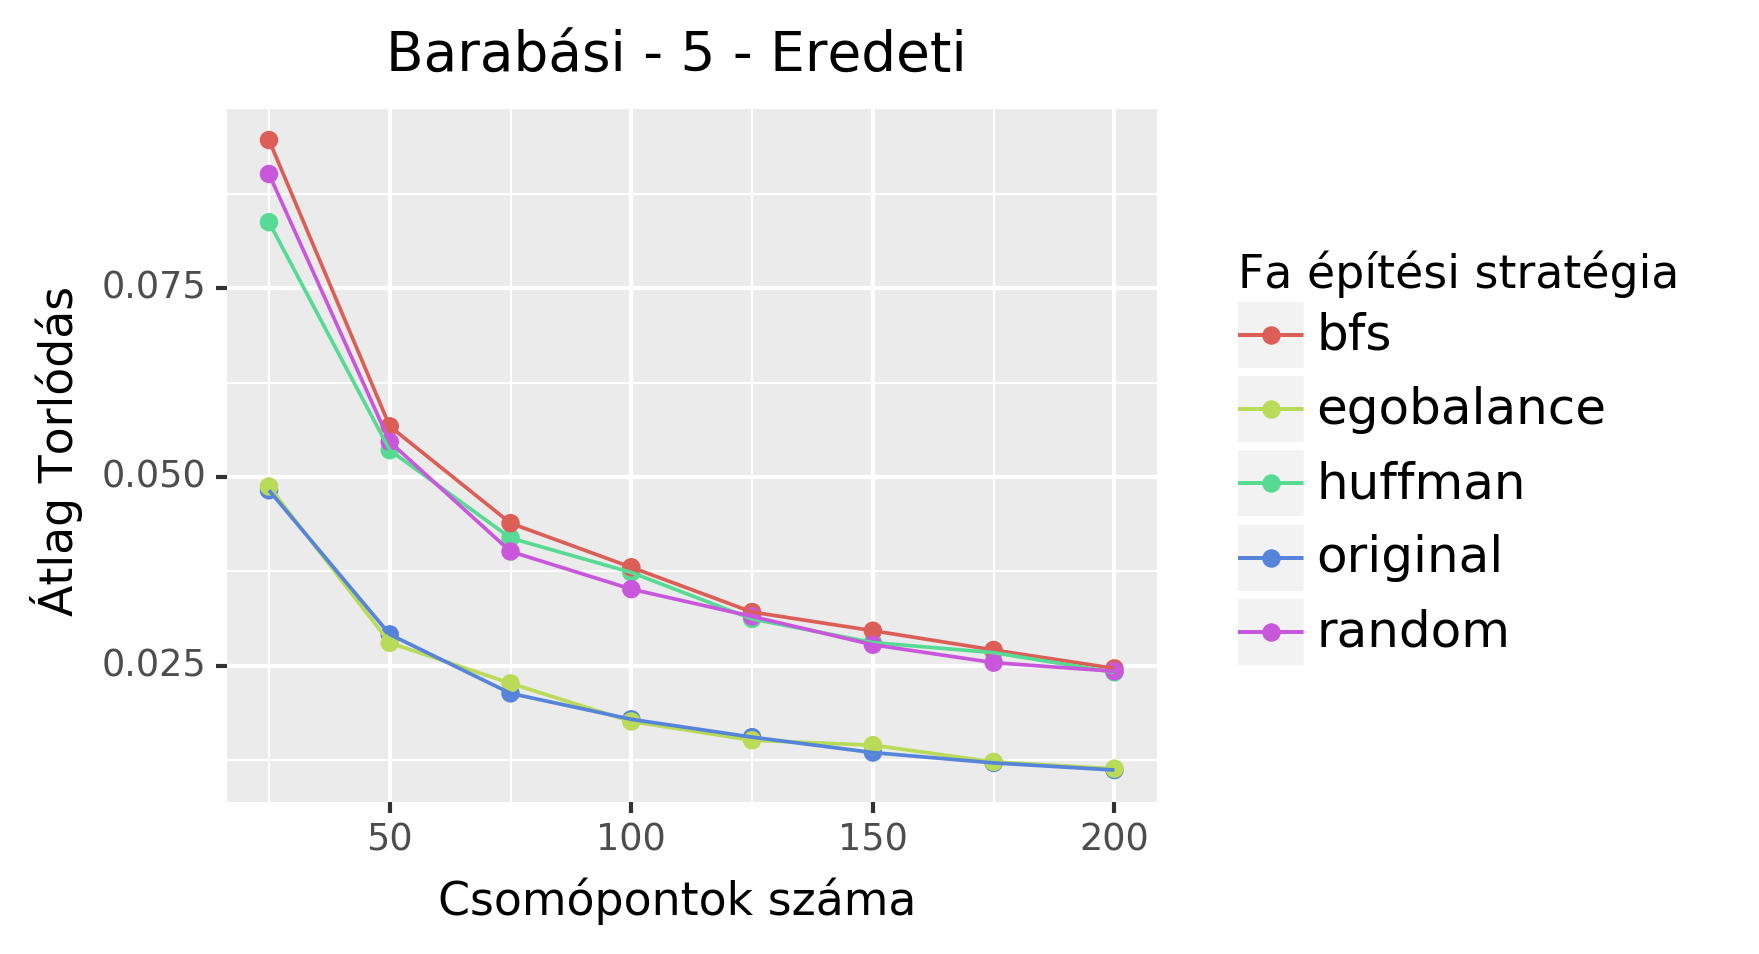
\includegraphics[width=0.49\linewidth]{pictures/barabasi_con_e.png}
		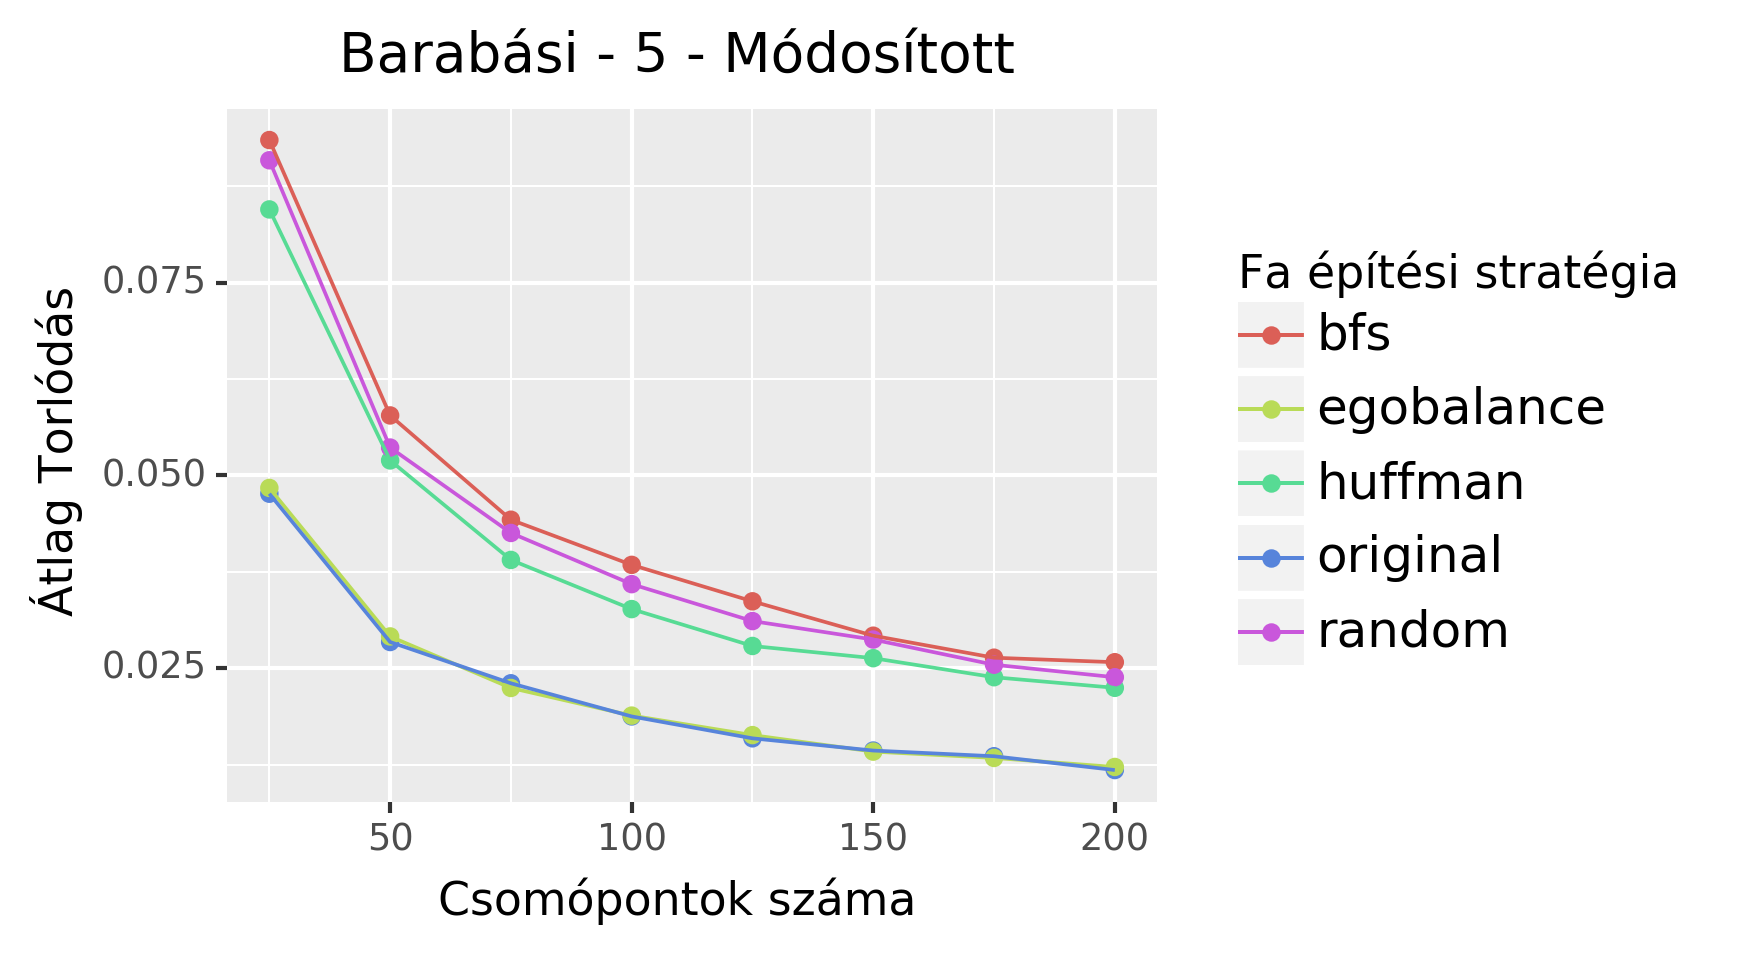
\includegraphics[width=0.49\linewidth]{pictures/barabasi_con_m.png}
		\caption{Barabási-Albert gráf - Fa számosság összehasonlítás}
		\label{barabasi-tree-difference-con}
	\end{center}
\end{figure}

Első jelentős különbség nem jelentkezik.

Következő gráfunk az Erdős-Rényi gráf a \ref{erdos-tree-difference-con} ábrán.

\begin{figure}[H]
	\begin{center}
		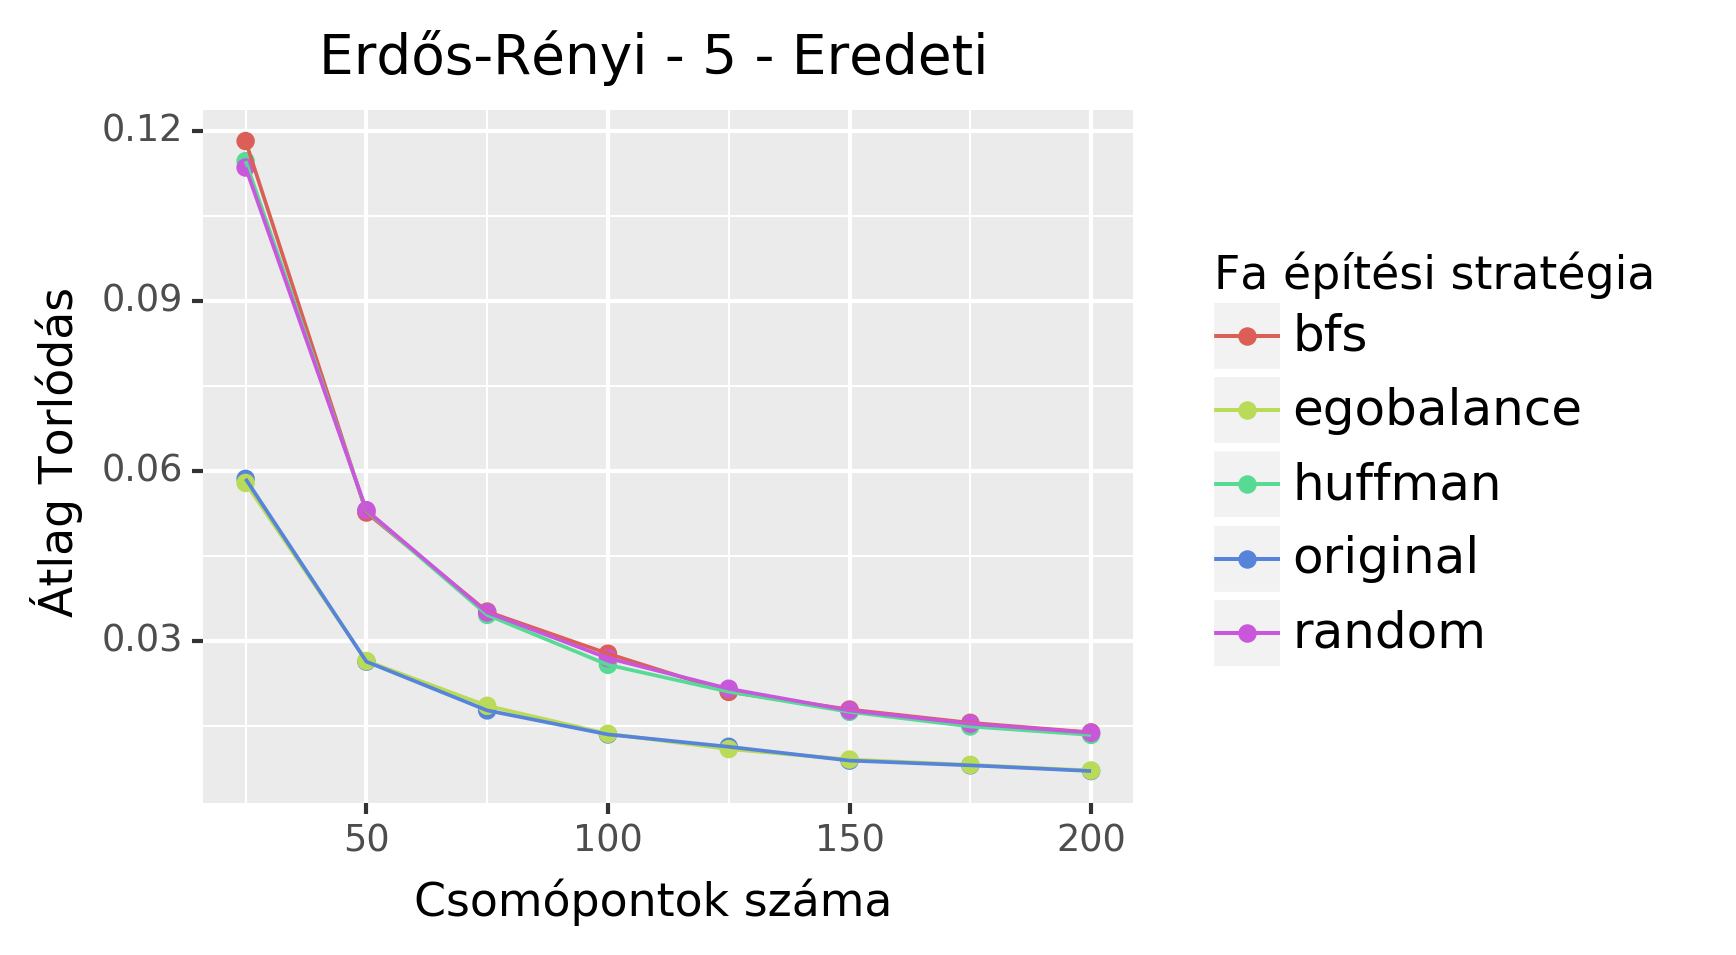
\includegraphics[width=0.49\linewidth]{pictures/erdos_con_e.png}
		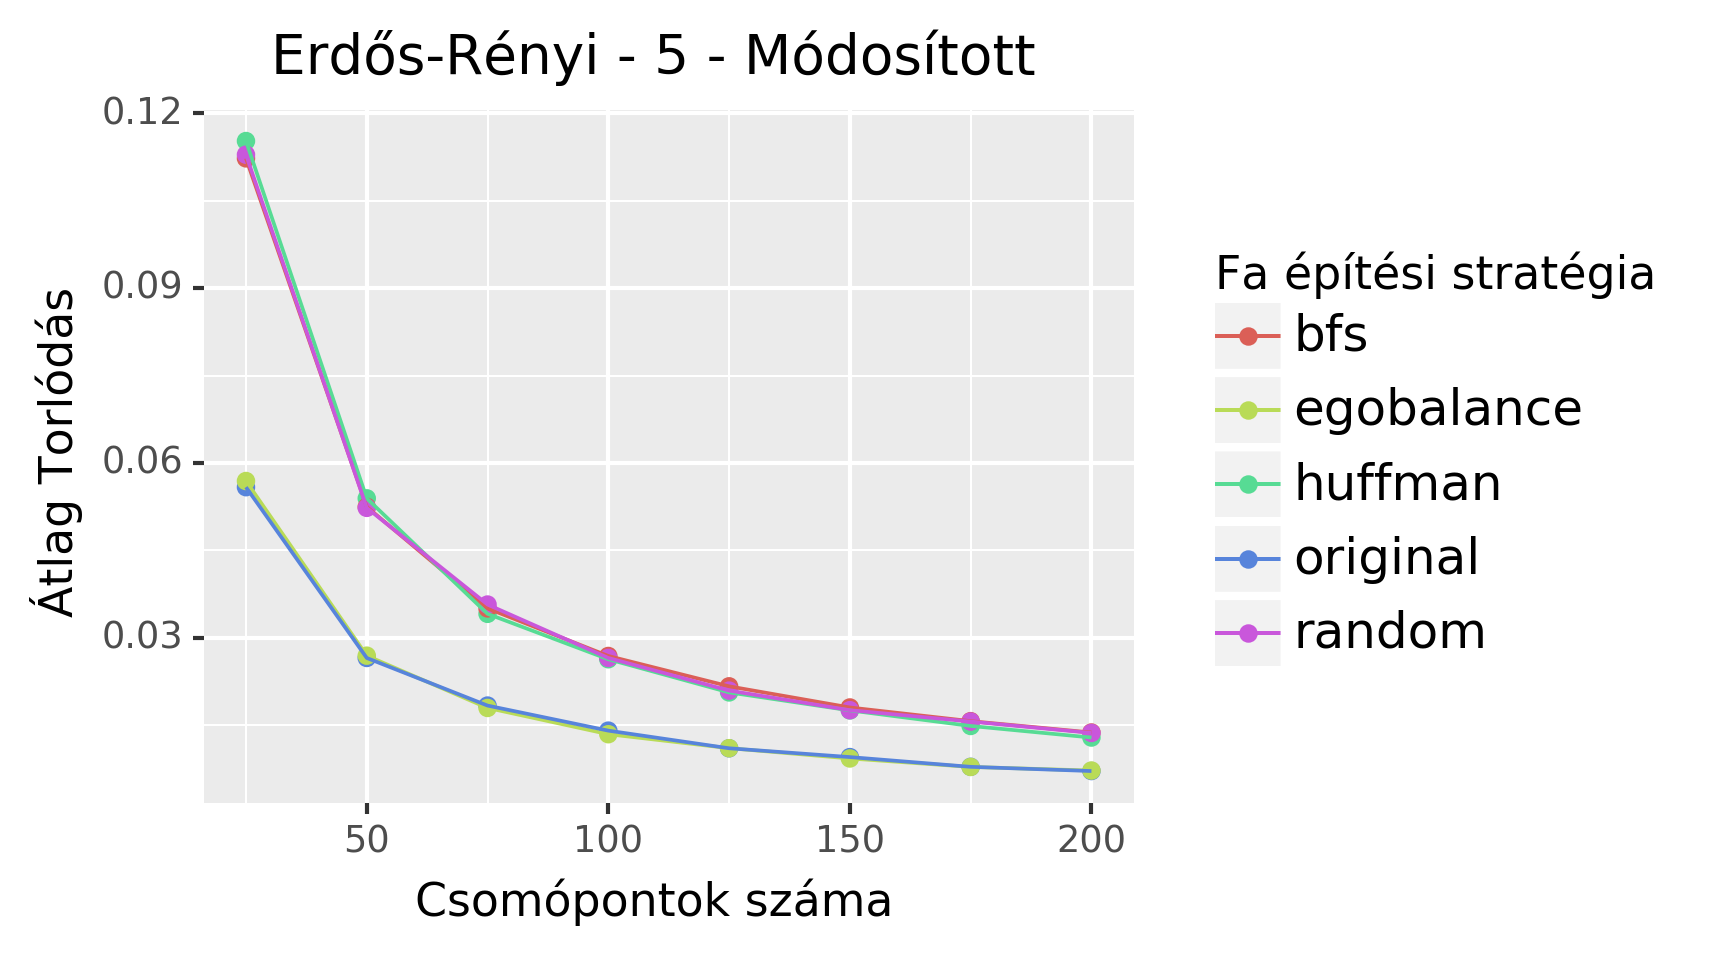
\includegraphics[width=0.49\linewidth]{pictures/erdos_con_m.png}
		\caption{Erdős-Rényi gráf - Fa számosság összehasonlítás}
		\label{erdos-tree-difference-con}
	\end{center}
\end{figure}

Jelentős különbség itt sem figyelhető meg.

Végül nézzük meg a csillag gráfot a \ref{star-tree-difference-con} ábrán. 

\begin{figure}[H]
	\begin{center}
		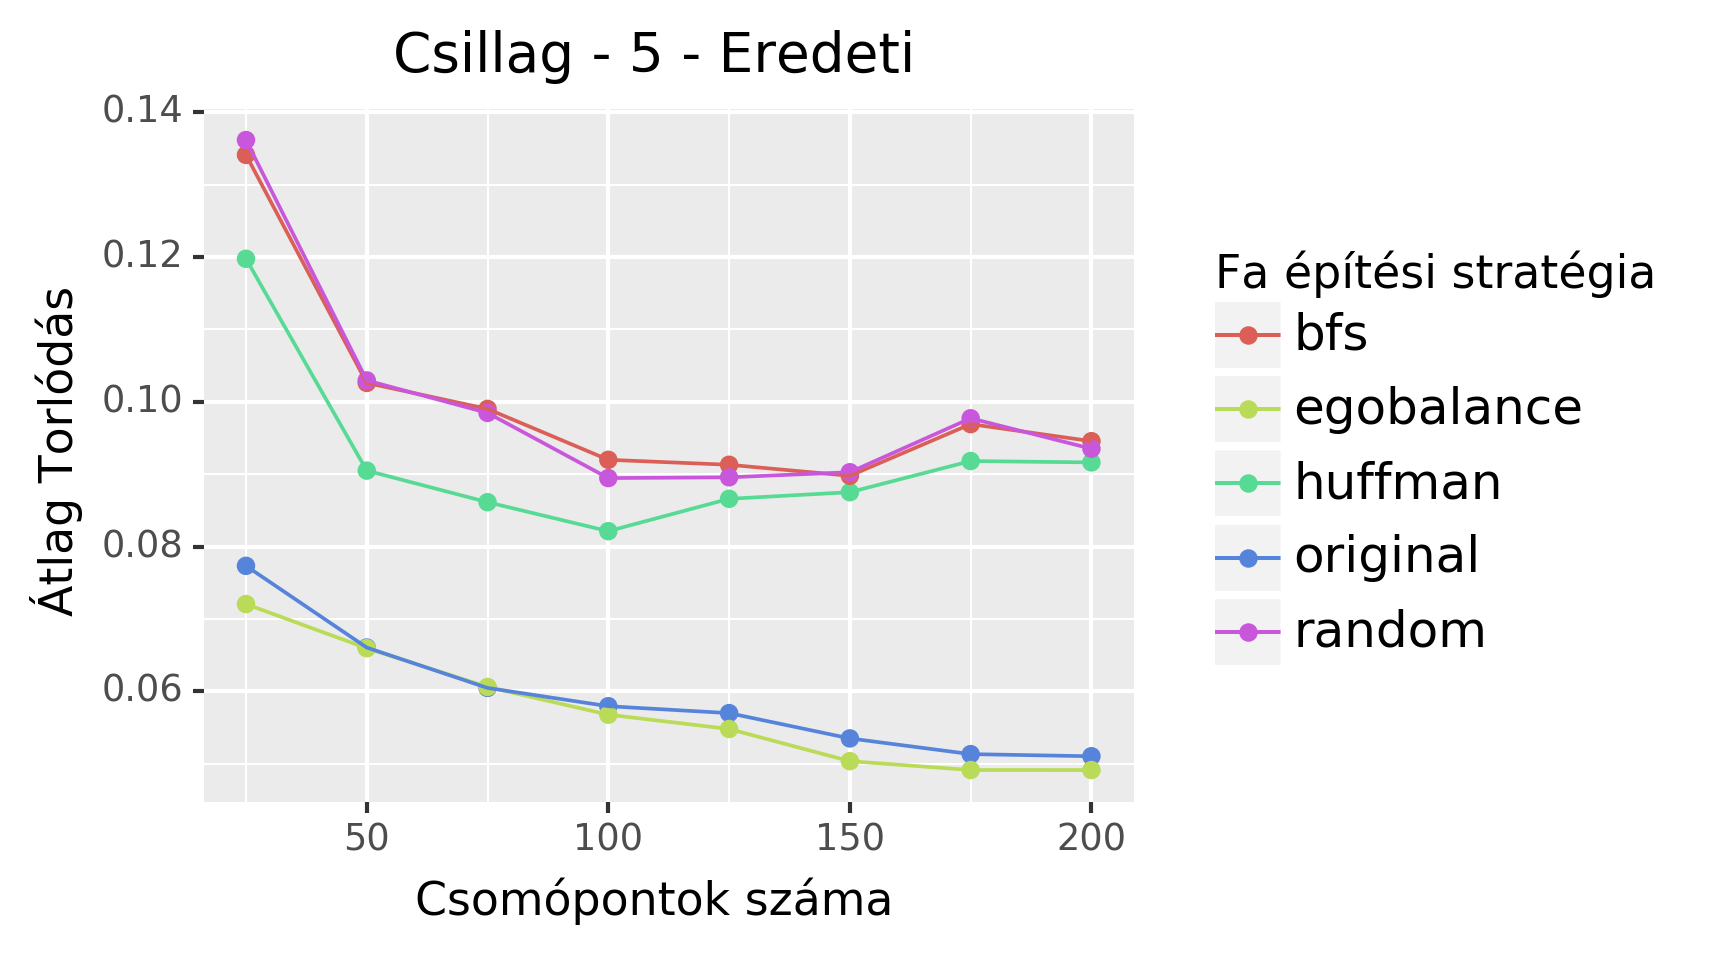
\includegraphics[width=0.49\linewidth]{pictures/star_con_e.png}
		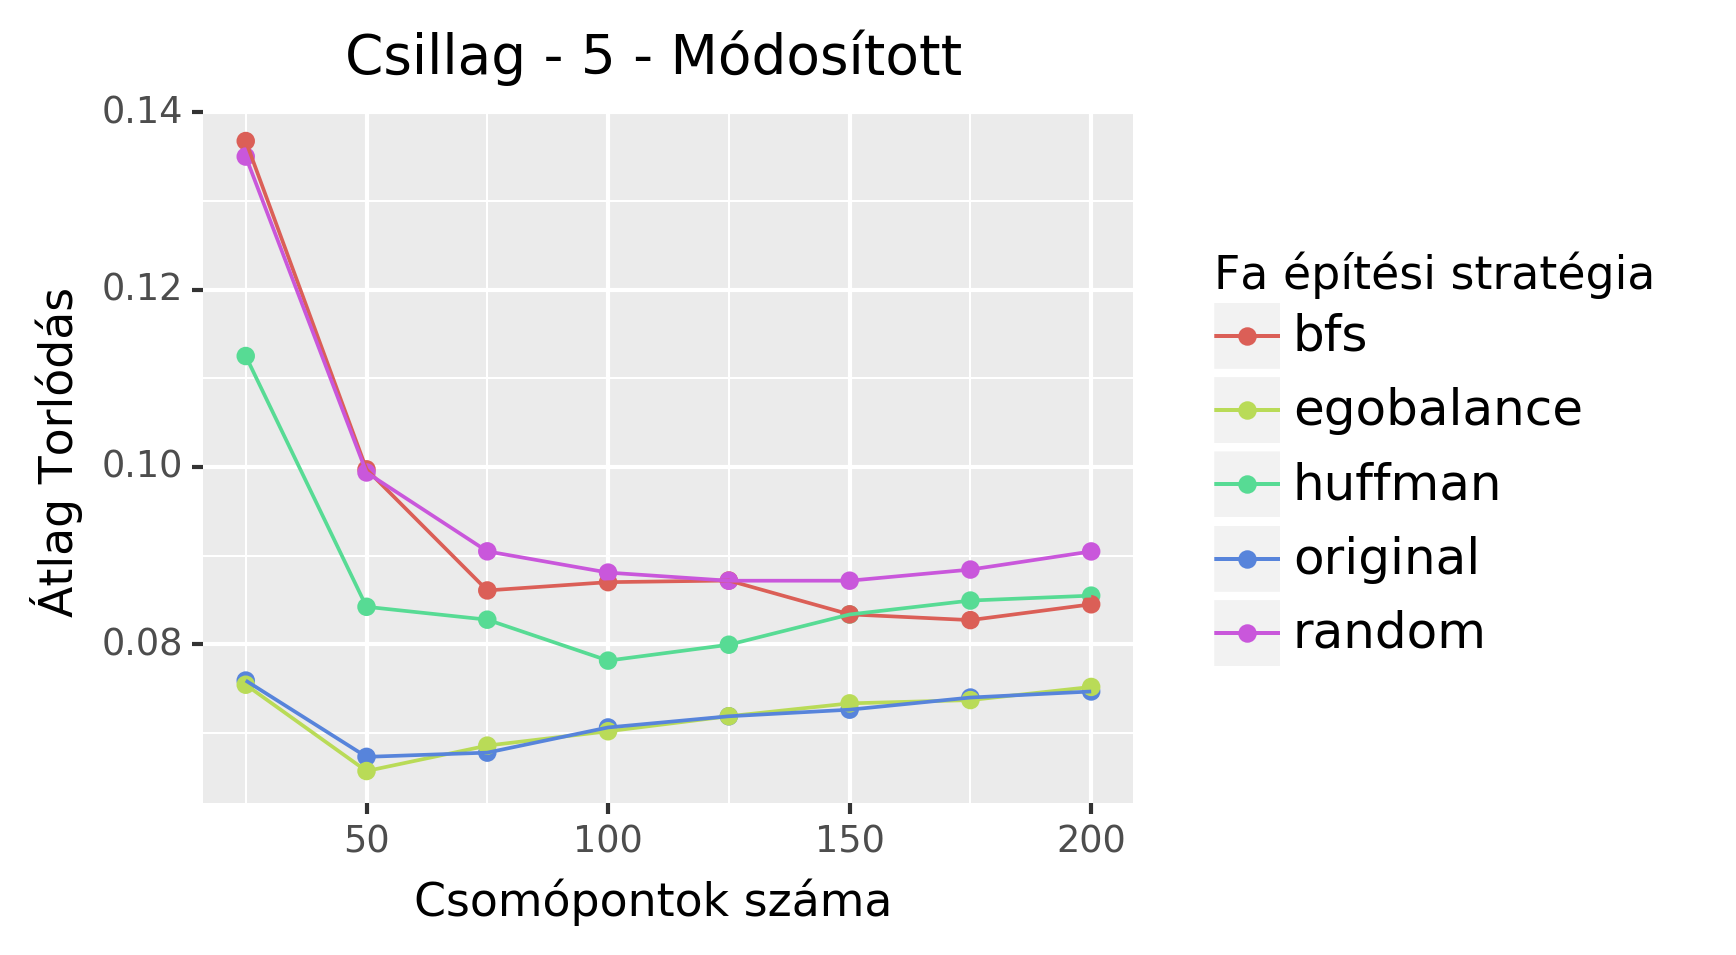
\includegraphics[width=0.49\linewidth]{pictures/star_con_m.png}
		\caption{Csillag gráf - Fa számosság összehasonlítás}
		\label{star-tree-difference-con}
	\end{center}
\end{figure}

Itt már jelentkezik különbség, az elején még hasonló a két gráf, de ahogy növeljük a csomópontok számát, a módosított algoritmus rosszabb eredményt eredményez, mint az eredeti algoritmus.

\chapter{Összefoglalás}

\section{Labor eredménye}

\subsection{Random fa algoritmus}

A Random fa algoritmusa nem lett a legjobb algoritmus az összes közül, de egy érdekes tényre mutatott rá.
A teljes fa építése mindig rövidebb utat eredményez, mintha különböző hosszúságú ágak lennének a fában torlódástól függően.
Ezért ez az algoritmus mindig jobb eredményt adott úthosszra, mint a cikkben megfogalmazott.
Mikor torlódáshoz értük, akkor egyértelműen látszik, hogy a véletlen szerűen összekapcsolt pontok nem lesznek torlódás optimálisak.
Az algoritmus alapját a Sorfolytonos fa adta, ezért mindkettő algoritmus szinte ekvivalens eredményhez vezetett.
 
\subsection{A fák számosságának hatása}

A labor lényegi kérdés az volt, hogy ha csak tényleg a szükséges fákat építjük meg akkor jobb lesz-e a hálózatunk.
A kapott eredményekből pedig az látszik, igen jobb lesz az úthossz esetében, mivel az algoritmus mindig rövidebb úthosszt eredményez, mint az eredeti.
Az torlódás már kicsit érdekesebb eredményt mutat, mivel a torlódásra nincs feltétlen kihatással, ha egy kiegyensúlyozott gráfot nézünk.
Ellenben, ha ez nem teljesül, hanem egy extrém esetet veszünk, a csillag gráfot, ott egyenesen rosszabb lesz az eredmény.

\section{A munka eredménye}

A cikk által meghatározott algoritmus megfelel arra, hogy teljesítse a célját, közel optimális útválasztási sémát készítsen egy ritka forgalmi mátrixszal reprezentált hálózathoz.
Attól függően, hogy értelmezzük a cikk egyes részeit, mikor csere lépést alkalmazzuk, kaphatunk két algoritmust, az Eredetit vagy az EgoBalance-t.
A kettő közötti különbség többnyire mérési hiba, ezért mindkettő elfogadható.
A másik három algoritmus is hasonló eredménnyel végzett, ami közül a Sorfolytonos fa egy befutó, ha a rövid utakat akarunk elérni minden áron.
Az épített fák mennyiség is egy fontos tényező, mivel jelentős úthossz csökkenéshez vezet, tolódás szempontjából pedig csak elfajult esetekben lesz rosszabb mint az eredeti algoritmus.
% Futás idő szempontjából a kevesebb fa kisebb futási időhöz vezet.

\bibliographystyle{abbrv}
\bibliography{refrences}

	
\end{document}